\chapter{Approximation method}
\section{Time independent perturbation theory}
\subsection{Brillouin-Wigner perturbation theory}
We consider an unperturbed Hamiltonian $H_0$ with eigenvalues $\epsilon_k$ and eigenstates $|k\alpha\rangle$, where $\alpha$ is an index introduced to resolve degeneracies, so that
\[H_0 |k\alpha\rangle = \epsilon_k |k\alpha\rangle\]
We pick one of these levels $\epsilon_n$ for study, so the index $n$ will be fixed for the following discussion. We denote the eigenspace of the unperturbed system corresponding to eigenvalue  $\epsilon_n$ by $\mathcal{H}$, so that the unperturbed eigenkets
$\{ |n\alpha\rangle, \alpha = 1,2,\cdots\}$ form a basis in this space.\\
We take the perturbed Hamiltonian to be $H = H_0 + \lambda H_1$, where $\lambda$ is a formal expansion parameter that we allow to vary between $0$ and $1$ to interpolate between the unperturbed and perturbed system. When the perturbation is turned on, the unperturbed energy level $\epsilon_n$ may split and shift. We denote one of the exact energy levels that grows out of $\epsilon_n$ by $E$. We let $|\psi\rangle$ be an exact energy eigenket corresponding to energy $E$, so that
\[H|\psi\rangle = (H_0 + \lambda H_1)|\psi\rangle = E|\psi\rangle\]
Both $E$ and $|\psi\rangle$ are understood to be functions of $\lambda$; as $\lambda \to 0$, $E$ approaches $\epsilon_n$ and $|\psi\rangle$ approaches some state lying in $\mathcal{H}_n$. We break the Hilbert space into the subspace $\mathcal{H}_n$ and its orthogonal complement which we denote by $\mathcal{H}_n^{\bot}$. The components of $|\psi\rangle$ parallel and perpendicular to $\mathcal{H}_n$ are conveniently expressed in terms of the projector $P$ onto the subspace $\mathcal{H}_n$ and the orthogonal projector $Q$, defined by
\[P = \sum_{\alpha} |n\alpha\rangle \langle n\alpha| \quad Q = \sum_{k \neq n,\alpha} |k\alpha\rangle \langle k\alpha|\]
These projectors satisfy
\[P^2=P \quad Q^2=Q \quad PQ=QP=0 \quad P+Q=I \quad [P,H_0]=[Q,H_0]=0\]
The component $P|\psi\rangle$ is a linear combination of the known unperturbed eigenstates $\{ |n\alpha\rangle, \alpha = 1,2,\cdots\}$, and is easily characterized. 
The orthogonal component $Q|\psi\rangle$ is harder to find. It turns out it is possible to write a neat power series expansion for this solution. Firstly, we have
\[(E-H_0)|\psi\rangle = \lambda H_1 |\psi\rangle\]
Now we define a new operator $R$
\[R \equiv \sum_{k \neq n,\alpha} \frac{|k\alpha\rangle \langle k\alpha|}{E-\epsilon_k}\]
\begin{note}
If there are other unperturbed energy levels $\epsilon_k$ lying close to $\epsilon_n$, then the perturbation could push
the exact energy $E$ near to or past some of these other levels, and then other small denominators would make $R$ ill defined.
This will certainly happen if the perturbation is large enough. For the time being we will assume this does not happen, so that $R$ is free of small denominators. When this is not the case we shall refer to "nearly degenerate perturbation theory", which is discussed later.
\end{note}
\noindent
The operator $R$ satisfies
\[PR=RP=0 \quad QR=RQ=R \quad R(E-H_0) = (E-H_0)R = Q\]
Then we have
\[R(E-H_0)|\psi\rangle = Q|\psi\rangle = \lambda RH_1 |\psi\rangle\]
and
\[|\psi\rangle = P|\psi\rangle + \lambda R H_1 |\psi\rangle\]
$|\psi\rangle$ can be solved as a series of $P|\psi\rangle$:
\[|\psi\rangle = \frac{1}{1-\lambda RH_1} P|\psi\rangle = P|\psi\rangle + \lambda RH_1P|\psi\rangle + \lambda^2 RH_1RH_1 P|\psi\rangle + \cdots\]

\subsection{Nondegenerate perturbation theory}
In nondegenerate perturbation theory the level $\epsilon_n$ of $H_0$ is nondegenerate. Then the index $\alpha$ is not needed for the level $\epsilon_n$, and we can write simply $|n\rangle$ for the corresponding eigenstate. We assume that $P|\psi\rangle$ is normalized rather than $\psi\rangle$ so that
\[P|\psi\rangle  = |n\rangle\]
With this normalization convention, we have
\[\langle n | \psi \rangle = 1\]
Now the series becomes
\[|\psi\rangle = |n\rangle + \lambda \sum_{k\neq n,\alpha} |k\alpha\rangle \frac{\langle k\alpha | H_1 | n \rangle}{E-\epsilon_k} + \lambda^2 \sum_{k\neq n,\alpha} \sum_{k'\neq n,\alpha'} |k\alpha\rangle \frac{\langle k\alpha | H_1 | k'\alpha' \rangle \langle k'\alpha' | H_1 | n \rangle}{(E-\epsilon_k)(E-\epsilon_{k'})}\]
To find an equation for $E$, we have
\[\langle n | E-H_0 | \psi\rangle = E-\epsilon_n = \lambda \langle n | H_1 | \psi\rangle\]
then we can get
\begin{eqnarray}
E &=& \epsilon_n + \lambda \langle n | H_1 | n\rangle + \lambda^2 \langle n | H_1RH_1 | n\rangle + \lambda^3 \langle n | H_1RH_1RH_1 | n\rangle + \cdots \nonumber \\
&=& \epsilon_n 
+ \lambda \langle n | H_1|n\rangle 
+ \lambda^2 \sum_{k\neq n,\alpha}  \frac{\lambda \langle n | H_1|k\alpha\rangle \langle k\alpha | H_1 | n \rangle}{E-\epsilon_k} \nonumber \\
&+& \lambda^3 \sum_{k\neq n,\alpha} \sum_{k'\neq n,\alpha'} \frac{\langle n | H_1 |k\alpha\rangle \langle k\alpha | H_1 | k'\alpha' \rangle \langle k'\alpha' | H_1 | n \rangle}{(E-\epsilon_k)(E-\epsilon_{k'})} + \cdots \nonumber
\end{eqnarray}
It is easy to get $E$ up to $O(\lambda^3)$,
\[E = \epsilon_n  + \lambda \langle n | H_1|n\rangle  + \lambda^2 \sum_{k\neq n,\alpha}  \frac{\lambda \langle n | H_1|k\alpha\rangle \langle k\alpha | H_1 | n \rangle}{\epsilon_n-\epsilon_k} + O(\lambda^3)\]
and $|\psi\rangle$ up to $O(\lambda^2)$,
\[|\psi\rangle = |n\rangle + \lambda \sum_{k\neq n,\alpha} |k\alpha\rangle \frac{\langle k\alpha | H_1 | n \rangle}{\epsilon_n-\epsilon_k} + O(\lambda^2)\]
\href{https://en.wikipedia.org/wiki/Perturbation_theory_(quantum_mechanics)#Second-order_and_higher_corrections}{Higher corrections} can be found on the internet.

\subsection{Degenerate perturbation theory}
In the case that the unperturbed energy level $\epsilon_n$ is degenerate, we have
\[P|\psi\rangle = \sum_{\alpha} |n\alpha\rangle c_{\alpha}\]
and
\[\langle n\alpha | P |\psi\rangle = \langle n\alpha  |\psi\rangle = c_{\alpha}\]
Then we can obtain an equation for the $c_{\alpha}$,
\[\langle n\alpha | E-H_0 | \psi\rangle = c_{\alpha}(E-\epsilon_n) = \lambda \langle n\alpha | H_1 | \psi\rangle\]
then we can get
\begin{eqnarray}
(E-\epsilon_{n})c_{\alpha} &=& \lambda \sum_{\beta} \langle n\alpha | H_1 | n\beta\rangle c_{\beta} + \lambda^2 \sum_{\beta} \langle n\alpha | H_1RH_1 | n\beta\rangle c_{\beta} + \cdots \\
&=& \lambda \sum_{\beta} \langle n\alpha | H_1 | n\beta\rangle c_{\beta}
+ \lambda^2 \sum_{\beta} \sum_{k\neq n,\gamma}  \frac{\lambda \langle n\alpha | H_1|k\gamma\rangle \langle k\gamma | H_1 | n\beta \rangle}{E-\epsilon_k}c_{\beta} + \cdots \nonumber
\end{eqnarray}
This equation must be solved simultaneously for the eigenvalues $E$ and the unknown expansion coefficients $c_{\alpha}$.\\
If we truncate the series at first order, we see that the corrections $E-\epsilon_{n}$ to the energies are determined as the eigenvalues of the matrix $\langle n\alpha | H_1 | n\beta\rangle$, and the coefficients $c_{\alpha}$ are the corresponding eigenvectors.
This determines the energies to first order, but the coefficients $c_{\alpha}$ only to zeroth order. Then $P|\psi\rangle$ becomes known to zeroth order and $Q|\psi\rangle$ to first order.\\
The first order matrix may or may not have degeneracies itself. If it does not, then all degeneracies are lifted at first order; if it does, the remaining degeneracies may be lifted at a higher order, or may persist to all orders. Degeneracies that persist to all orders are almost always due to some symmetry of the system, which can usually be recognized at the outset.\\
The higher order corrections can be calculated step by step, which will not be listed here.\\ \\
Now let us consider the case in which the unperturbed levels of $H_0$ , while not technically degenerate, are close to one another. Suppose to be specific that two levels, say, $\epsilon_n$ and $\epsilon_m$, are close enough to one another that first order perturbations will push the exact level $E$ close to or onto the unperturbed level $\epsilon_m$.\\
In this case we choose some energy, call it $\bar{\epsilon}$, which is close to $\epsilon_n$ and $\epsilon_m$. Then let us take the original unperturbed Hamiltonian and perturbation and rearrange them in the form,
\[H = H_0 + H_1 = H'_0 + H'_1\]
where
\begin{eqnarray}
H_0 &=& \sum_{k\alpha} \epsilon_k |k\alpha\rangle\langle k\alpha| \nonumber \\
H'_0 &=& \sum_{k\neq m,n; \alpha} \epsilon_k |k\alpha\rangle\langle k\alpha| + \sum_{k= m,n; \alpha} \bar{\epsilon} |k\alpha\rangle\langle k\alpha| \nonumber \\
H'_1 &=& H_1 + \sum_{k= m,n; \alpha} (\epsilon_k - \bar{\epsilon} )|k\alpha\rangle\langle k\alpha| \nonumber
\end{eqnarray}
Then standard degenerate perturbation theory may be applied.
We will call this procedure "nearly degenerate perturbation theory."

\section{Application of time independent perturbation theory in hydrogen atom}
\subsection{Stark effect}
The Stark effect concerns the behaviour of atoms in external electric fields. We choose hydrogen atom because it is single-electron atoms.
The hydrogen atom will be modelled with the central force Hamiltonian
\[H_0 = \frac{p^2}{2m} - \frac{e^2}{4\pi r}\]
In this Hamiltonian we ignore spin and other small effects such as relativistic corrections, hyperfine effects and the Lamb shift. These effects cause a splitting and shifting of the energy levels of our simplified model, as well as the introduction of new quantum numbers and new degrees of freedom.
But these effects are all small, and if the applied electric field is strong enough, it will overwhelm them and the physical consequences will be much as we shall describe them with our simplified model. \\
The unperturbed energy levels in hydrogen are given by
\[E_n = -\frac{1}{2n^2} \frac{e^2}{4\pi a_0}\]
where $a_0$ is the Bohr radius. These levels are $n^2$ degenerate.\\
As for the perturbation, let us write $\bm{F}$ for the external electric field , and let us take it to lie in the z-direction. Thus, the perturbing potential has the form
\[V_1 = -(-e)\bm{F}\cdot\bm{x} = eFz\]
For small $z$, the attractive Coulomb field dominates the total potential and we have the usual Coulomb well that supports atomic bound states. However, for large negative $z$, the unperturbed potential goes to zero, while the perturbing
potential becomes large and negative. At intermediate values of negative $z$, the competition between the two potentials gives a maximum in the total potential. The electric force on the electron is zero at the maximum of the potential. 
Given the relative weakness of the applied field, the maximum must occur at a distance from the nucleus that is large in comparison to the Bohr radius $a_0$. Atomic states with small principal quantum numbers $n$ lie well inside this radius. The perturbation analysis we shall perform applies to these states.\\
The bound states of the unperturbed system are able to tunnel through the potential barrier. When an external electric field is turned on, the bound states of the atom cease to be bound in the strict sense, and become resonances. 
Electrons that tunnel through the barrier and emerge into the classically allowed region at large negative $z$ will accelerate in the external field, leaving behind an ion. This is the phenomenon of field ionization. This effect can be neglected if the external field is weak enough and the lifetime of the "bound state" is long enough.\\ \\
In the case of hydrogen, the ground state is $|100\rangle$. The first order shift in the ground state energy level is given by
\[\Delta E^{(1)}_{gnd} = \langle 100 | eFz | 100\rangle = 0\]
which vanishes because the parity of $z$ is odd, but $\langle 100 |$ and $| 100\rangle$ have the same parity.\\
For the excited states of hydrogen, according to first order degenerate perturbation theory, the shifts in the energy levels $E_n$ are given by the eigenvalues of the $n^2\times n^2$ matrix,
\[\langle nlm | eFz | nl'm'\rangle\]
According to the Wigner-Eckart theorem and parity, the matrix elements vanish unless $l -l' = \pm 1$ and $m = m'$. Consider, for example, the case $n=2$. The four degenerate states are  $|2,0,0\rangle$, $|2,1,-1\rangle$, $|2,1,0\rangle$ and $|2,1,1\rangle$. Only the states $|2,0,0\rangle$ and $|2,1,0\rangle$ are connected by the perturbation. Therefore of the $16$ matrix elements, the only nonvanishing ones are
\[\langle 2,0,0 | eFz | 2,1,0\rangle = -W = -3eFa_0\]
and its complex conjugate. The matrix connecting the two states $|2,0,0\rangle$ and $|2,1,0\rangle$ is
\[\begin{pmatrix}0 & -W \\ -W & 0\end{pmatrix} \]
and its eigenvalues are the first order energy shifts in the $n=2$ level,
\[\Delta E_2^{(1)} = \pm W\]
In addition, the two states $|2,1,-1\rangle$ and $|2,1,1\rangle$ do not shift their energies at first order. The perturbed eigenfunctions are
\[|+W\rangle = \frac{|2,0,0\rangle - |2,1,0\rangle}{\sqrt{2}} \quad |-W\rangle = \frac{|2,0,0\rangle + |2,1,0\rangle}{\sqrt{2}}\]
This is zeroth order part of the exact eigenstates.\\
Now let us look at the exact symmetries of the full, perturbed Hamiltonian $ H = H_0 + H_1$, without doing perturbation theory at all. Since $[H,L_z]$ the exact eigenstates of $H$ can be chosen to be eigenstates of $L_z$ as well.
Denote these by $|\gamma m \rangle$, where $\gamma$ is an additional index needed to specify an energy
eigenstate. Thus, we have
\[L_z |\gamma m \rangle = m |\gamma m \rangle \quad H |\gamma m \rangle = E_{\gamma m} |\gamma m \rangle\]
where $E_{\gamma m}$ is allowed to depend on $m$ since the full rotational symmetry is broken. \\
As for time reversal, the state $T|\gamma m\rangle$ must be an eigenstate of energy with eigenvalue $E_{\gamma m}$ since $TH = HT$. But because $T^{-1}L_zT = -L_z$, it also follows that $T|\gamma m\rangle$ is an eigenstate of $L_z$ with eigenvalue $-m$ . If $m \neq 0$, we must have a degeneracy of at least two. 
The only energy levels that can be nondegenerate are those with $m=0$. In the example above, even higher order corrections cannot separate $|2,1,-1\rangle$ and $|2,1,1\rangle$.

\subsection{Fine structure}
Fine structure of atoms concerns the effects of relativity and spin on the dynamics of the electron. Both these effects are of the same order of magnitude, and must be treated together in any realistic treatment of the atomic structure.\\
The fine structure terms account for relativistic effects through order $v^2$ , and have the effect of enlarging the Hilbert space by the inclusion of the spin degrees of freedom, introducing new quantum numbers, and shifting and splitting the energy levels of the electrostatic model. 
The splitting in particular means that spectral lines that appear a singlets under low resolution become closely spaced multiplets under higher resolution.\\
Derivation of the exact form of relativistic corrections of Hamiltonian in quantum mechanics can be very rigorous and needs some reasonable guess. The details of derivation can be found in 
\href{http://bohr.physics.berkeley.edu/classes/221/1112/notes/finestruc.pdf}{lecture notes on fine structure} by Robert G. Littlejohn. Here we just list the result.
\[H_{FS} = H_{RKE} + H_{D} + H_{SO}\]
The term $H_{RKE}$ is due to the second order term of the expansion series of $E = \sqrt{p^2+m^2}$. (The first order term is just the kinetic energy in non relativistic quantum mechanics). We have
\[H_{RKE} = - \frac{p^4}{8m^3}\]
The term $H_{D}$ comes out as a result of virtual process $e^{-} \to e^{-} + e^{-} + e^{+}$ in the region whose is scale is smaller than the Compton length $\lambda_C = \frac{1}{m} = \alpha a_0$ of electrons. Such virtual states appear in perturbation theory when one sums over intermediate states, which derive ultimately from a resolution of the identity. The effect is to smear out the position of the atomic electron
over a distance of order $\lambda_C$. We have
\[H_D = \frac{1}{8m^2} \nabla^2 V\]
The term $H_{SO}$ arises because the electric field of nuclei generates a magnetic field in the rest frame of electron. We have
\[H_{SO} = \frac{1}{2m^2} \frac{1}{r} \frac{dV}{dr} \bm{L}\cdot\bm{S}\]
The unperturbed energy levels in hydrogen are given by
\[E_n = -\frac{1}{2n^2} \frac{e^2}{4\pi a_0}\]
When spin of electron is taken into account,  these levels are $2n^2$ degenerate. One choice of base is $|nlm_{l}s\rangle$. It is the eigenvector of operator $L^2$, $L_z$ and $S_z$. However, $L_z$ and $S_z$ do not commute with $H_{SO}$. A better choice of base is $|nljm_j\rangle$. It is the eigenvector of operator $L^2$, $J^2$ and $J_z$. $H_{SO}$, $H_{RKE}$ and $H_{SO}$ are all commute with $L^2$, $J^2$ and $J_z$. So
\[\langle n l' j' m'_j | H | n l j m_j\rangle\]
vanishes unless $l'=l$, $j=j'$ and $m'_j = m_j$. The final results are
\[\langle n l j m_j | H_{RKE} | n l j m_j\rangle = -\alpha^2 E_n \frac{1}{n^2} \left(\frac{3}{4} - \frac{n}{l+\frac{1}{2}} \right)\]
\[\langle n l j m_j | H_{D} | n l j m_j\rangle = -\alpha^2 E_n \frac{1}{n}\delta_{l0}\]
\[\langle n l j m_j | H_{SO} | n l j m_j\rangle = -\alpha^2 E_n \frac{1}{2n} \frac{j(j+1)-l(l+1)-\frac{3}{4}}{l(l+\frac{1}{2})(l+1)}\]
When we add them up to get the total energy shift due to the fine structure we find
\[\Delta E_{FS} = -\alpha^2 E_n \frac{1}{n^2} \left(\frac{3}{4} - \frac{n}{j+\frac{1}{2}} \right)\]
It is independent of the orbital angular momentum quantum number $l$, although each of the individual terms does depend on $l$. However, the total energy shift does depend on $j$ in addition to the principal quantum number $n$, so when we take into account the fine structure corrections, the energy levels of hydrogen atom have the form $E_{nj}$.\\ \\
Besides fine structure effect, the remaining important effects causing energy shift are hyperfine effects and the Lamb shift.\\
The Lamb shift is a shift in the energy levels due to the interaction of the electron with the vacuum fluctuations of the quantized electromagnetic field. It has small effects on the s-states ($l = 0$) of hydrogen, thereby introducing a dependence of the energy levels on $l$. Thus, including the Lamb shift, the energy levels in hydrogen have the form $E_{nlj}$ , and the only degeneracy is that due to rotational invariance. It will be further discussed in quantum electrodynamics.\\
Hyperfine effects are caused by the interaction between electro spin and nuclei spin, and will be discussed later.

\subsection{Zeeman effect}
The Zeeman effect concerns the interaction of atomic systems with external magnetic fields. The Hamiltonian for the electron in hydrogen atom is
\[H = \frac{(\bm{P}+e\bm{A})^2}{2m} - \frac{e^2}{4\pi r} + H_{FS} + g_e \mu_B\bm{S}\cdot\bm{B}\]
where $g_e \approx 2$ and $\mu_B \equiv \frac{e}{2m}$.
We assume a uniform magnetic field $\bm{B} = B\hat{\bm{z}}$. We take the gauge
\[\bm{A} = \frac{1}{2}\bm{B}\times\bm{r}\]
which is Coulomb gauge so that $\bm{\nabla}\times\bm{A} = 0$. This implies
\[\bm{P}\cdot\bm{A} = \bm{A}\cdot\bm{P}\]
so the cross terms in the expansion of the kinetic energy can be written in either order. We also notice that
\[\bm{P}\cdot\bm{A} = \frac{1}{2} \bm{P}\cdot\bm{B}\times\bm{r}  = \frac{1}{2}\bm{B}\cdot\bm{L}\] 
At last, we have
\[H = H_a + H_Z + H_B + H_{FS}\]
where
\[H_a = \frac{p^2}{2m} - \frac{e^2}{4\pi r} \quad  H_Z = \frac{e}{2m}(L_z + 2S_z)B \quad H_B = \frac{e^2}{8m}B^2(x^2+y^2)\]
Suppose the typical energy of the term $H_{i}$ is $E_i$, then we have $E_a \sim \frac{me^4}{32 n^2 \pi^2\hbar^2\epsilon_0^2}$, $E_z \sim \frac{ne\hbar B}{2m}$ and $E_B \sim \frac{e^2}{8m}n^4 a_0^2 = \frac{2n^4\pi^2 \epsilon_0^2 \hbar^4 B^2}{m^3 e^2}$. So
\[\frac{E_Z}{E_a} \sim \frac{16\pi^2 n^3 \hbar^3 \epsilon_0^2}{m^2 e^3} B \sim \frac{n^3B}{2\times10^5 T}\]
\[\frac{E_B}{E_a} \sim \left[ \frac{8\pi^2 n^3 \hbar^3 \epsilon_0^2}{m^2 e^3} B\right]^2 \sim \left[ \frac{n^3B}{4\times10^5 T} \right]^2\]
In the previous section, we have derived that
\[\frac{E_{FS}}{E_a} \sim \frac{3\alpha^2}{4n^2} \sim \frac{1}{2.5\times10^4 n^2}\]
So,in the usual experimental condition, we have
\[E_B \ll E_z \ll E_a\]
So, in the following discussion, we will neglect $E_B$ term.
But whether $\frac{E_{FS}}{E_Z}$ is much larger than $1$, much smaller than $1$ or close to $1$ depends on the $B$ and $n$.\\ \\
If $H_{FS}$ is much smaller than $H_Z$ and can be neglected, then we have
\[H = H_a + \frac{e}{2m}(L_z + 2S_z)B\]
The eigenvector of $H$ is $|nlm_lm_s\rangle$ with eigenvalue $E = E_n + \mu_B B(m_l+2m_s)$.
\begin{figure}[!h]
	\centering
	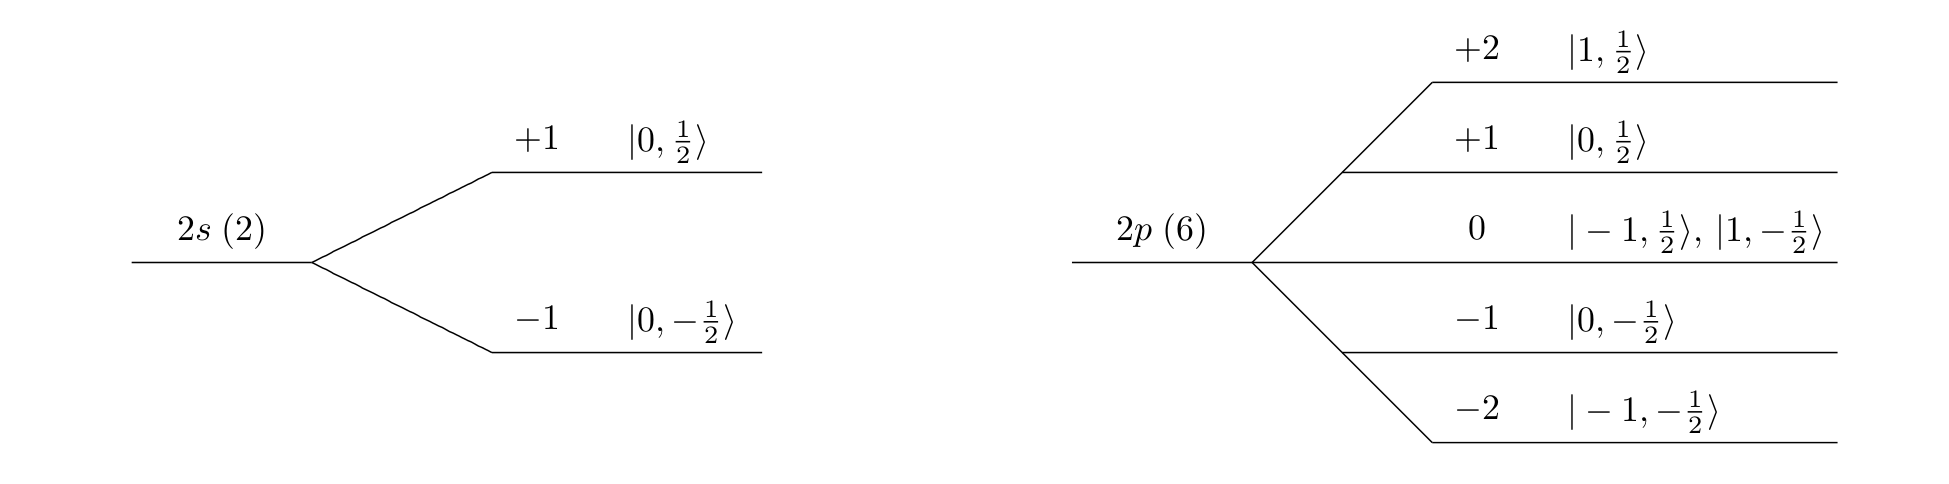
\includegraphics[height=4cm ,width=16cm]{QM/zeeman1.png}
	\caption{Zeeman effect for $n=2$ in Hydrogen atom}
\end{figure}\\
If $H_{FS}$ is much smaller than $H_Z$ and but cannot be neglected, we may treat it as a perturbation. For simplicity, we only take $H_{SO}$ into account. Up to the first order, we consider the matrix element
\[\langle n l m_l m_s | f(r)\bm{L}\cdot\bm{S}| n l' m'_l m'_s\rangle\]
Since $[H_{SO},L^2] = 0$, the term above vanishes unless $l = l'$. So we focus on the matrix in the subspace $l = l'$. For the $2p$ orbit of hydrogen, there is a 2-fold degeneracy between $|2,1,-1,\frac{1}{2}\rangle$ and $|2,1,1,-\frac{1}{2}\rangle$.
This makes one $2 \times 2$ matrix. Let us look at the off-diagonal element,
\[\langle 2,1,-1,\frac{1}{2} | f(r)\bm{L}\cdot\bm{S}| 2,1,1,-\frac{1}{2}\rangle\]
in which we use the identity
\[\bm{L}\cdot\bm{S} = \frac{1}{2}(L_+S_-+L_-S_+)+L_zS_z\]
To be non-vanishing, the operator in the middle of the matrix element must connect states with $\Delta m_l = 2$, but in fact that operator permits only $\Delta_m = 0,\pm1$. Therefore the off-diagonal matrix element vanishes and the energy shift is determined by diagonal elements. For $2p$ orbit, we can get
\[\Delta E = \langle n l m_l m_s | f(r)\bm{L}\cdot\bm{S}| n l m_l m_s\rangle \propto m_lm_s\]
As for the $2s$ levels, for them $\bm{L} = 0$ (that is, the operator $\bm{L}$ vanishes on the 2s-subspace), so $\Delta E = 0$.\\ \\
The final case we shall examine is the weak field limit, in which $H_z \ll H_{FS}$ and we will treat $H_z$ as perturbation.
\begin{note}
In the case of hydrogen, one should also consider the Lamb shift for a realistic treatment. For example, in the $n=2$ levels of hydrogen, the Lamb shift is about $10$ times smaller than the fine structure energy shifts, indicating that we really should question how the Lamb shift compares to the Zeeman term which is also (by our assumptions) much smaller than the fine structure term.
\end{note}
\noindent
The eigenvector of $H_a + H_{FS}$ are $|nljm_j\rangle$ with eigenvalue $E_{nj}$. Up to the first order,the matrix elements we need have the form
\[\langle n l' j m'_j | H_z | n l j m_j\rangle\]
Since $[H_Z,L^2] = 0$ and $[H_Z,J_z] = 0$, off-diagonal matrix element vanishes automatically.The energy shift is
\[\Delta E = \mu_B B\langle n l j m_j | L_z + 2S_z | n l j m_j\rangle = g_{eff} \mu_B B m_j\]
where
\[g_{eff} = 1 + \frac{j(j+1)-l(l+1)+s(s+1)}{2j(j+1)}\]

\subsection{Hyperfine structure}
The nucleus of an atom contains localized charge and current distributions, which produce electric and magnetic fields that can be decomposed into multipole fields much as in classical electrostatics or magnetostatics.
The first of the multipole moments, the electric monopole, is of course the Coulomb electrostatic field that holds the electrons in their orbits and produces the gross structure of the atom.
The higher order multipole moments produce small corrections to the atomic structure that are known generally as hyperfine effects.\\
Multipole moments for a system of charges has been discussed in the part of classical electrodynamics. In quantum mechanics, we recall that the intrinsic magnetic moment operator of an electron is defined in the space of electron spin. So we may infer that multipole moments of nuclei is defined in the space of nuclear spin $\bm{I}$. 
We let the quantum number of the operator $I^2$ be $i$, so that $I^2$ has eigenvalues $i(i+1)$. The nuclear Hilbert space is a  $(2i+1)$ dimensional space in which the standard basis is $|im_i\rangle$ with $-i \leq m \leq i$.\\
Not all the multipole fields that occur classically are allowed in the case of a nuclei. There are two rules governing the allowed multipole moments of the nucleus.\\ 
The first is that electric multipoles of odd $k$ and magnetic mutlipoles of even $k$ are forbidden. For example, if the nucleus had an electric dipole moment, the perturbing Hamiltonian would be
\[H_1 = -e \frac{\bm{d}\cdot\bm{r}}{r^3}\]
And just like $\bm{\mu}$,$\bm{d}$, must be proportional to the spin, say $\bm{d} = k\bm{I}$, because all vector operators on a single irreducible subspace are proportional (Wigner-Eckart theorem). Thus,
\[H_1 = -ke \frac{\bm{I}\cdot\bm{r}}{r^3}\]
We find that $H_1$ violates time reversal and parity
\[T H_1 T^{\dagger} = -H_1 \quad P H_1 P^{\dagger} = -H_1\]
The weak interactions do violate parity, and we do know that time reversal (more precisely, CP) is violated at a very small  level in certain decay processes, so it is possible that the terms forbidden by this rule actually exist at a small level. For example, the neutron or the electron may have an electric dipole moment, but if such moments exist, they are certainly very small and can be neglected in our discussion.\\
The second rule states that a $2^k$-pole can occur only if $k \leq 2i$. For example, the proton with $i = \frac{1}{2}$ can possess an electric monopole moment and a magnetic dipole moment, but not an electric quadrupole moment. Lying behind this rule is the fact that the operator representing the $2^k$ -pole on the nuclear Hilbert space is, in fact, an order $k$ irreducible tensor operator. But the maximum order of an irreducible tensor operator on the nuclear Hilbert space with
spin $i$ is $k = 2i$.\\
So for hydrogen atom, whose nuclear spin is $i = \frac{1}{2}$, the only term we have to concern is magnetic moment. A point magnetic dipole of moment $\bm{\mu}$ is
\[\bm{A}(\bm{r}) = \frac{\bm{\mu}\times\bm{r}}{r^3}\]
To avoid the sigularuty at origin, we modify $\bm{A}(\bm{r})$ as
\[\bm{A}(\bm{r}) = \bm{\mu}\times\bm{r} \begin{cases} \frac{1}{a^3} \quad r < a\\ \frac{1}{r^3} \quad r > a\end{cases} \]
taking into account of the finite size of nuclei. 
By taking the curl we compute the magnetic field
\[\bm{B}(\bm{r}) =  \begin{cases} \frac{2\bm{\mu}}{a^3} \quad r < a\\ \bm{\mu}\cdot\hat{T} \quad r > a\end{cases} \]
where $T_{ij} = \frac{3x_ix_j-r^2\delta_{ij}}{r^5}$
We define
\[\Delta(r) \equiv \begin{cases} \frac{1}{a^3} \quad r < a\\ 0 \quad r > a\end{cases}\]
and
\[f(r) \equiv \begin{cases} 0 \quad r < a\\ 1 \quad r > a\end{cases}\]
Then we can write
\[\bm{A}(\bm{r}) = \bm{\mu}\times\bm{r} \left [\Delta(r) + \frac{f(r)}{r^3}\right ] \]
and
\[\bm{B}(\bm{r}) = \bm{\mu}\cdot \left [2\Delta(r)\hat{I} + f(r)\hat{T}\right ] \]
In the limit $a \to 0$, we have
\[\lim_{a \to 0} \Delta(r) = \frac{4\pi}{3}\delta(\bm{r}) \quad \lim_{a \to 0} f(r) = 1\]\\
The Hamiltonian of the system is
\[H = \frac{(\bm{p}+e\bm{A})^2}{2m} - \frac{e^2}{4\pi r} + H_{FS} + H_{Lamb} + \frac{e}{m}\bm{S}\cdot{B}\]
The expressions  for $\bm{A}$ and $\bm{B}$ are are given above and $\bm{\mu}$ in the expression are given by
\[\bm{\mu} = g_{p} \mu_p \bm{I}\]
where $g_p$ is g-factor of proton and $\mu_p \equiv \frac{e}{2m_p}$. Thus, the Hamiltonian must be interpreted as an operator acting the total Hilbert space
\[\mathcal{H} = \mathcal{H}_{elec} \otimes \mathcal{H}_{nucl}\]
For $\mathcal{H}_{elec}$ the obvious basis is $|nljm_j\rangle$ with energies $E_{nlj}$ when there is no hyperfine terms. In hydrogen energies depend on $l$ because of the Lamb shift. The obvious basis in $\mathcal{H}_{nucl}$ is $|im_i\rangle$. Thus we define the basis states in $\mathcal{H}$ as $|nljm_jm_i\rangle$ (we suppress the index $i$ since it is a constant).It is called uncoupled basis. Now we expand the Hamiltonian and neglect the term $A^2$, writing the result as $H = H_0 + H_1$ , where
\[H_0 = \frac{p^2}{2m} - \frac{e^2}{4\pi r}  + H_{FS} + H_{Lamb}\]
and
\[H_1 = 2\mu_B(\bm{p}\cdot{A} + \bm{S}\cdot\bm{B})\]
Since
\[\bm{p}\cdot(\bm{I}\cdot{r}) = \bm{I}\cdot(\bm{r}\cdot{P}) = \bm{I}\cdot\bm{L}\]
we have
\[H_{1,orbi} \equiv 2\mu_B(\bm{p}\cdot\bm{A}) = k(\bm{I}\cdot\bm{L}) \left[\Delta(r) + \frac{f(r)}{r^3}\right ]\]
where $k \equiv = g_eg_p\mu_B\mu_p$.
On the other hand, we have
\[H_{1,spin} \equiv 2\mu_B \bm{S}\cdot\bm{B} = k\left [2\Delta(r)\bm{I}\cdot\bm{S} + f(r)\bm{I}\cdot\hat{T}\cdot\bm{S}\right ] \]
In the limit $a \to 0$, we have
\[H_{1,orbi} = k(\bm{I}\cdot\bm{L}) \left[\frac{4\pi}{3}\delta(\bm{r}) + \frac{1}{r^3}\right ]\]
and
\[H_{1,spin}  = k\left [\frac{8\pi}{3}\delta(\bm{r})\bm{I}\cdot\bm{S} + \bm{I}\cdot\hat{T}\cdot\bm{S}\right ] \]
Since the coupling term (e.g.$\bm{I}\cdot{S}$) are not invariant under either electronic rotations alone or under nuclear rotations alone. The uncoupled basis is not the best one for carrying out the perturbation calculation. The total angular momentum of the system are defined by
\[\bm{F} \equiv \bm{I} + \bm{J} = \bm{I} + \bm{L} + \bm{S}\]
The new coupled basis is $|nljfm_f\rangle$. Since $[\bm{F},H] = 0$, $|nljfm_f\rangle$ is the eigenvector of $H$. The energy shift caused by $H_1$ is
\[\Delta E = \langle nljfm_f | H_1 | nljfm_f\rangle\]
After a lengthy calculation, we can get
\[\Delta E = \frac{g_eg_p\mu_B\mu_p}{4\pi a_0^3} \frac{1}{n^3} \frac{f(f+1)-j(j+1)-i(i+1)}{j(j+1)(2l+1)} \]
The energy levels were $E_{nlj}$ before the hyperfine interactions were turned on, but since $\Delta E$ depends on $f$, they now have the form $E_{nljf}$ . The energy eigenstates are $|nljfm_f\rangle$, and are $(2f+1)$-fold degenerate, causing the fine structure levels of hydrogen to split, giving rise to hyperfine multiplets. \\
For example, the ground state $|1,0,\frac{1}{2}\rangle$ splits into two levels $f = 0$ and $f = 1$. This $f = 0$ level is the true ground state of hydrogen. It is nondegenerate. The $f=1$ level is 3-fold degenerate, and lies above the ground state by an energy of approximately $1.42 GHz$ in frequency
units, or $21 cm$ in wave length units.

\section{Time dependent perturbation theory}
\subsubsection{Dyson series}
Time-dependent perturbation theory applies to Hamiltonians of the form
\[H = H_0 + H_1(t)\]
where $H_0$ is solvable and $H_1$ is treated as a perturbation.In time-dependent perturbation theory, we are usually interested in time-dependent transitions between eigenstates of the unperturbed system induced by the perturbation $H_1$.
Time-dependent transitions are usually described by the transition amplitude, defined as the quantity
\[\langle f | U(t) | i \rangle\]
where $U(t)$ is the exact time evolution operator for the Hamiltonian, and where $|i\rangle$ and $|f\rangle$ are
two eigenstates of the unperturbed Hamiltonian $H_0$. 
Let us denote the unperturbed time-evolution operator by $U_0(t)$ and the exact one by $U(t)$.
These operators satisfy the evolution equations
\[i\frac{\partial U_0(t)}{\partial t} = H_0U_0(t) \quad i\frac{\partial U(t)}{\partial t} = HU(t)\]
Since $H_0$ is independent of time, we have $U_0 = e^{-iH_0 t}$.\\ \\
Suppose the state in Schrödinger picture is $|\psi_S(t)\rangle$, then we define the state in interaction picture as
\[|\psi_I(t)\rangle \equiv U^{\dagger}_0(t) |\psi_S(t)\rangle\]
Similarly, we define the operator in interaction picture as
\[A_I(t) \equiv U^{\dagger}_0(t) A_S(t) U_0(t)\]
Let us define $W(t)$ as the operator that evolves kets in the interaction picture forward from time $0$ to final time $t$, i.e.
\[ |\psi_I(t)\rangle = W(t) |\psi_I(0)\rangle \]
We can verify that
\[W(t) = U^{\dagger}_0U(t)\]
And we can get the time evolution of $W(t)$
\[i\frac{\partial W}{\partial t} = H_{1I}(t)W(t)\]
The formal solution is
\[W(t) = I + (-i)^n \sum_{n=1}^{\infty} \int_{0}^{t}dt_1 \int_{0}^{t_1}dt_2 \cdots \int_{0}^{t_{n-1}} dt_n H_{1I}(t_1)H_{1I}(t_2)\cdots H_{1I}(t_n)\]\\
Let us assume for simplicity that $H_0$ has a discrete spectrum $H_0|n\rangle = E_n|n\rangle$. 
We assume that the system is initially in an eigenstate of the unperturbed system, what we will call the "initial" state $|i\rangle$ with energy $E_i$. Then 
\[|\psi_I(t)\rangle = W(t)|i\rangle\]
Let us expand the exact solution of the Schrödinger equation in the interaction picture in the unperturbed eigenstates
\[|\psi_I(t)\rangle = \sum_n c_n(t) |n\rangle\]
We then have
\[c_n(t) = \langle n | W(t) | i\rangle = \langle n | U^{\dagger}_0U(t) | i\rangle = e^{iE_nt} \langle n | U(t) | i\rangle \]
So the transition amplitudes in the interaction picture and those in the Schrödinger picture are related by a simple phase factor.The transition probabilities are the squares of the amplitudes and are the same in either case. The perturbation expansion of the transition amplitude $c_n(t)$ is
\[c_n(t) = \delta_{ni} + c^{(1)}_n(t) + \cdots\]
where
\[c^{(1)}_n(t) = \frac{1}{i} \int_0^t dt' \langle n | H_{1I}(t')|i\rangle = \frac{1}{i} \int_0^t dt' e^{i(E_n-E_i)t'} \langle n | H_{1}(t')|i\rangle\]

\subsubsection{Constant and harmonic perturbation}
If $H_1$ is time-independent, we have
\[c^{(1)}_n(t) = \frac{2}{i} e^{i\omega_{ni}t/2} \left( \frac{\sin\omega_{ni}t/2}{\omega_{ni}} \right) \langle n | H_1 | i \rangle\]
Up to the first order, the transition probability is
\[P_n(t) = 4 \left( \frac{\sin^2\omega_{ni}t/2}{\omega_{ni}^2} \right) |\langle n | H_1 | i \rangle|^2 \quad (n \neq i)\]\\
Another case that is important in practice is when $H_1$ has a periodic time dependence of the form
\[H_1(t) = Ke^{-i\omega_0t} + K^{\dagger}e^{i\omega_0t}\]
We can get
\[c^{(1)}_n(t) = \frac{2}{i} \left[ e^{i(\omega_{ni}-\omega0)t/2} \left( \frac{\sin(\omega_{ni}-\omega_0)t/2}{\omega_{ni}-\omega_0} \right) \langle n | K | i \rangle  + e^{i(\omega_{ni}+\omega_0)t/2} \left( \frac{\sin(\omega_{ni}+\omega_0)t/2}{\omega_{ni}+\omega_0} \right) \langle n | K^{\dagger} | i \rangle \right]  \]
Often, we are most interested in those final states to which most of the probability goes, which are the states for which one or the other of the two denominators is small.
For these states we have
\[E_n \approx E_i \pm \omega_0\]
We call these two cases absorption and stimulated emission, respectively. 
Taking the case of absorption, and looking only at final states that are near resonance, we can write the transition probability to first order of perturbation theory as
\[P_n(t) = 4 \left( \frac{\sin^2(\omega_{ni}-\omega_0)t/2}{(\omega_{ni}-\omega_0)^2} \right) |\langle n | K | i \rangle|^2\]

\subsubsection{Transition probability}
Let us fix the final state and examine how the probability develops as a function of time in first order time-dependent perturbation theory.
Obviously $P_n(0) = 0$. At later times we see that $P_n(t)$ oscillates at frequency $\omega_{ni}$ between $0$ and a maximum proportional to $\frac{1}{\omega_{ni}}$.
The frequency $\omega_{ni}$ measures how far the final state is off resonance, that is, how much it fails to conserve energy. If this frequency is large, the probability oscillates rapidly between zero and a small maximum. 
But as we move the state closer to the initial state in energy, $\omega_{ni}$ gets smaller, the period of oscillations becomes longer, and the amplitude grows.\\
If there is a final state degenerate in energy with the initial state, then $\omega_{ni}=0$ and the time-dependent factor takes on its limiting value $\frac{t^2}{4}$. In this case, first order perturbation theory predicts that the probability grows without bound. 
This is an indication of the fact that at sufficiently long times first order perturbation theory breaks down and we must take into account higher order terms in the perturbation expansion. But at short times it is correct that $P_n$ for a state on resonance grows as $t^2$.\\ \\
Now let us fix the time $t$ and examine how the expression for $P_n(t)$ in first order perturbation theory depends on the energy of the final state. To do this we focus on $\frac{\sin^2(\omega t/2)}{\omega^2}$ as a function of $\omega$.\\
The curve of the function consists of oscillations under the envelope $\frac{1}{\omega^2}$, with zeroes at $\omega = \frac{2n\pi}{t}$. The
central lobe has height $\frac{t^2}{4}$ and width that is proportional to $\frac{1}{t}$, so the area of the central lobe
is proportional to $t$. We can derive that
\[\lim_{t \to \infty} \frac{1}{t} \frac{\sin^2\omega t/2}{\omega^2} = \frac{\pi}{2}\delta(\omega)\]
The $\delta$-function enforces energy conservation in the limit $t \to \infty$. But at finite times, transitions take place to states in a range of energies about the initial energy.
This width is of order $\frac{1}{t}$. This is an example of
the energy-time uncertainty relation, $\Delta t \Delta E \sim 1$, indicating that a system that is isolated (not
subjected to a measurement) over a time interval $\Delta t$ has an energy that is uncertain by an amount $\Delta E \sim \frac{1}{\Delta t}$.\\
It is conventional to define the transition rate as the transition probability per unit time,i.e.
\[\Gamma(i \to f) = \lim_{t \to \infty}{P(i \to f)}{t}\]
Up to the first order, we have
\[\Gamma(i \to f) = 2\pi \delta(E_i - E_f) |V_{fi}|^2\]
where $V_{fi} = \langle f | H_1 | i \rangle$.

\section{Atomic Radiation}
We apply time-dependent perturbation theory to the interaction of atomic electron with the classical radiation field.
The basic Hamiltonian, with $A^2$ omitted, is
\[H = \frac{p^2}{2m} - e\phi(\bm{x}) + \frac{e}{m}\bm{A}\cdot\bm{p}\]
Specifically, we work with a linear polarized monochromatic field of the plane wave for
\[\bm{A} = 2A_0\bm{\epsilon}\cos(\bm{k}\cdot\bm{x}-\omega t) = A_0\bm{\epsilon} [e^{i\bm{k}\cdot\bm{x}}e^{-i\omega t}  + e^{-i\bm{k}\cdot\bm{x}}e^{i\omega t} ]\]
So, $\frac{e}{m}\bm{A}\cdot\bm{p}$ is a Harmonic perturbation with $K = \frac{eA_0}{m} e^{i\bm{k}\cdot\bm{x}} (\bm{\epsilon}\cdot\bm{p})$.
For example, take the case of absorption, the transition rate is
\[\Gamma(i \to f) = 2\pi \frac{e^2|A_0|^2}{m^2} |\langle f |e^{i\bm{k}\cdot\bm{x}} (\bm{\epsilon}\cdot\bm{p}) |i \rangle|^2 \delta(E_f-E_i-\omega)\]
The cross section can be calculated by the transition rate of absorption.\\ \\
The electrical dipole approximation is based on the fact that the wavelength of radiation field is far longer than the atomic dimension, so that the series
\[e^{i\bm{k}\cdot\bm{x}} = 1+ ii\bm{k}\cdot\bm{x}+\cdots\]
can be approximated by its leading term, $1$. Suppose the direction of the EM is wave is $z$, we now have
\[\langle f |e^{i\bm{k}\cdot\bm{x}} (\bm{\epsilon}\cdot\bm{p}) |i \rangle = \langle f | p_z |i \rangle = \frac{m}{i} \langle f |  [z,H_0] |i \rangle = im(E_n-E_i)\langle f | n |i \rangle  \]
where $H_0 = \frac{p^2}{2m} - e\phi(\bm{x})$.\\
Recall the Wigner-Eckart theorem, we have the selection rules: The matrix element would vanish unless $\Delta m = 0$ and $\Delta l = \pm 1$ ($\Delta l $ can be $0$ because parity consideration. Further more, if the EM wave is circular polarized, we would have $\Delta m = \pm 1$. If the fine structure is taken into account, we would have $\Delta j = 0,\pm 1$ and $\Delta l = \pm 1$. If the hyperfine structure is taken into account, we would have $\Delta f = 0,\pm 1$, $\Delta j = 0,\pm 1$ and $\Delta l = \pm 1$. 

\section{Variational Method}
Let $H$ be a Hamiltonian which is assumed to have some bound states. Let the discrete (bound state) energy eigenvalues be ordered $E_0 < E_1 < \cdots$. The eigenvalues are allowed to be degenerate. There may also be a continuous spectrum above some energy, as often happens in practice.\\
Let $|\psi\rangle$ be any normalizable state. Then the theorem states that
\[\frac{\langle \psi | H | \psi \rangle}{\langle \psi | \psi \rangle} > E_0\]
The state $|\psi\rangle$ is chosen to be an approximation to the ground state, based on physical intuition or other criteria, and the upper bound on $E_0$ that is obtained is often quite useful. \\
In practice we often choose a continuous family of trial wave functions. Let $\lambda$ be a continuous parameter, and let us write the family as $|\psi(\lambda)\rangle$. Then we define a function of $\lambda$, really an energy function,
\[F(\lambda) = \frac{\langle \psi(\lambda) | H | \psi(\lambda) \rangle}{\langle \psi(\lambda) | \psi(\lambda) \rangle}\]
We minimize this by finding the root $\lambda_0$ of
\[\frac{\partial F}{\partial \lambda} = 0\]
so that the best estimate to the ground state wave function out of the family is $|\psi(\lambda)\rangle$ and the best estimate for the ground state energy is $F(\lambda_0)$. 
Of course we must check that the root is actually a minimum.
\\ \\
In practice the normalization denominators are often inconvenient. One possibility is simply to normalize each member of the set of trial wave functions so those denominators are not
present. 
But often it is easier to enforce normalization by using Lagrange multipliers. We introduce the function,
\[F(\lambda,\beta) = \langle \psi(\lambda) | H | \psi(\lambda) \rangle - \beta (\langle \psi(\lambda) | \psi(\lambda) \rangle - 1)\]
and then require
\[\frac{\partial F}{\partial \lambda} = 0 \quad \frac{\partial F}{\partial \beta} = 0\]


\chapter{Many body problem}
\section{Identical particles}
If two particles are identical, their exchange must not change physical quantities, so we have
\[|\cdots\psi_j\cdots\psi_i\cdots\rangle = E_{ij}|\cdots\psi_i\cdots\psi_j\cdots\rangle = e^{i\theta} |\cdots\psi_i\cdots\psi_j\cdots\rangle\]
where $E_{ij}$ is the operator to exchange particle $i$ and $j$ and $psi_i$ is the quantum number to describe the state of particle $i$.
In coordinate representation, it can be expressed as
\[\Psi(\cdots\bm{x}_j\cdots\bm{x}_i\cdots) = e^{i\theta} \Psi(\cdots\bm{x}_i\cdots\bm{x}_j\cdots)\]
In three dimension space, the value of $e^{i\theta}$ can only be $\pm 1$. If the spin of the particle is integer, then the phase factor must be $1$ and the particle is called boson. If the spin of the particle is half-integer, then the phase factor must be $-1$ and the particle is called fermion. This is called spin-statistics theorem and can only be proved by relativistic quantum field theory. Here, we will take it for granted.
\begin{note}
In two dimension space, the phase $e^{i\theta}$ can be anything, and the particles that obey quantum statistics of this sort are called anyons. There is a brief introduction in chapter 12.1 and
12.2 of the book \emph{Quantum Field Theory and the Standard Model (Matthew D. Schwartz)}.
\end{note}
\noindent
So not all vectors in the space $\mathcal{H}_1\otimes\cdots\otimes\mathcal{H}_n$ are physical state. The physical states must be the eigenvectors of all $E_{ij}$ with eigenvalue $1$ ($-1$) for bosons (fermions). The space composed of physical states is the so-called Fock space. For example, suppose there are three particles with different state $a,b,c$. $|abc\rangle$ is not a physical state. The physical state for bosons is
\[\frac{1}{\sqrt{3!}} \left( |abc\rangle + |acb\rangle + |bca\rangle + |bac\rangle + |cab\rangle + |cba\rangle\right)\]
The physical state for fermions is
\[\frac{1}{\sqrt{3!}} \left( |abc\rangle - |acb\rangle + |bca\rangle - |bac\rangle + |cab\rangle - |cba\rangle\right)\]
In general, for $N$ particles filling $N$ distinct states, there are $N!$ states to start with, but there is only one totally symmetric state and one totally anti-symmetric state, and the rest of $N!-2$ states are thrown out. Therefore quantum statistics reduces the size of the Hilbert space quite dramatically.\\
Further more, not all Hermitian operators are physical observables. A nonphysical operator is one that takes a state
in the physical subspace of the Hilbert space (one that satisfies the right symmetry under exchange), and maps it into a nonphysical state (one that does not have the right symmetry).
An example is the operator $\bm{X}_1$. We might call this the operator corresponding to the measurement of the position of
particle 1. 
The problem with this operator from a physical standpoint is that you cannot measure the position of particle 1. You can select a region of space, and ask whether there is a particle in that region. But if you find one, you cannot say whether it is particle 1 or particle 2, since they are identical. 
If $O$ is a physical observables, we must have
\[[E_{ij},O] = 0\]
for all $ij$.
\begin{figure}[!h]
	\centering
	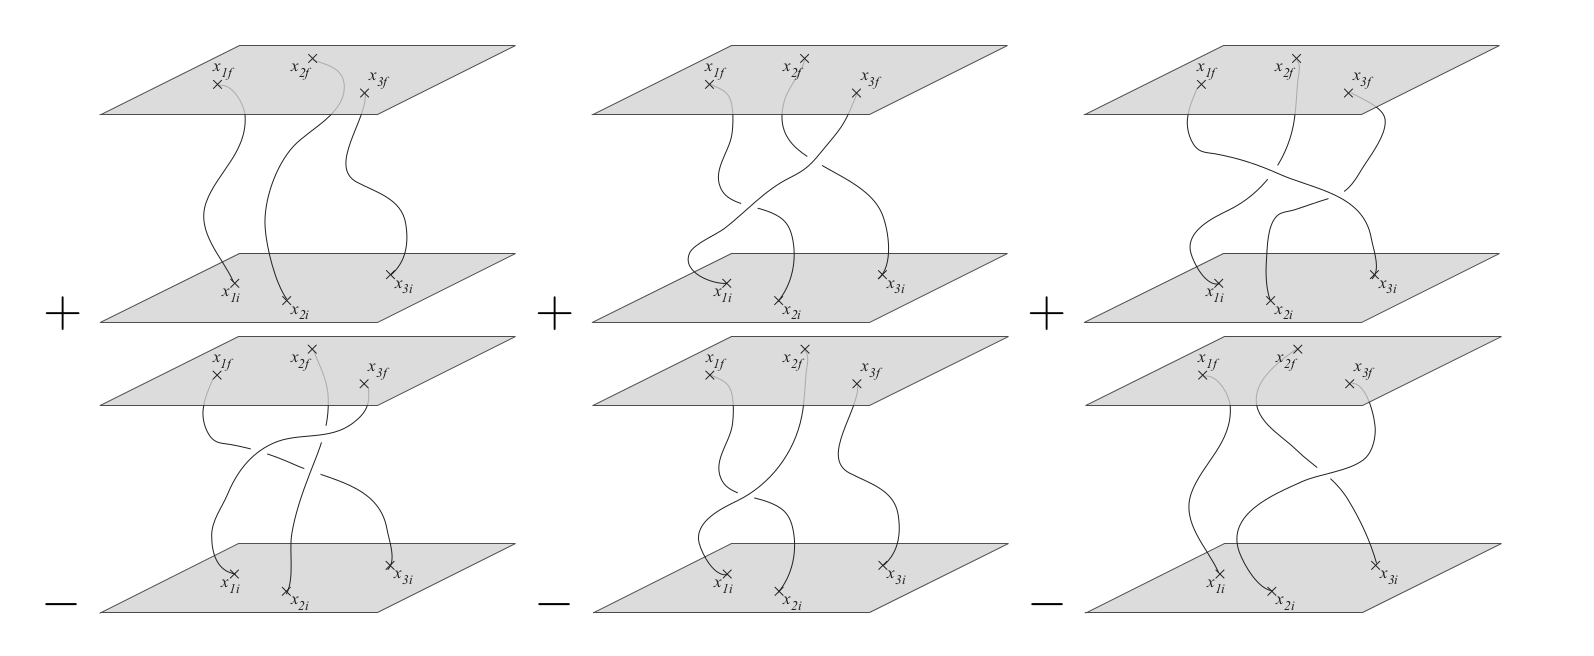
\includegraphics[height=4cm ,width=9.7cm]{QM/pathint.png}
	\caption{The path integral for three identical fermions}
\end{figure}\\
In path integral formulation of quantum mechanics, we calculate the transition amplitudes
\[\langle \bm{x}_f,t_f | \bm{x}_i,t_i\rangle = \int \mathcal{D}\bm{x}(t) e^{i\int_{t_i}^{t_f} dt L(t)}\]
The generalization to the N -particle case is
\[\langle \bm{x}_{1f}\cdots\bm{x}_{Nf},t_f | \bm{x}_{1i}\cdots\bm{x}_{Ni},t_i\rangle = \int \mathcal{D}\bm{x}_1(t)\cdots\bm{x}_N(t) e^{i\int_{t_i}^{t_f} dt L(t)}\]
Here, the particle 1 at the initial position $\bm{x}_{1i}$ moves to the final position $\bm{x}_{1f}$, the particle 2 at the initial position $\bm{x}_{2i}$ to $\bm{x}_{2f}$ , etc, and you sum over all possible paths.
When the particles are identical, however, we need to introduce proper (anti-)symmetry of the state. For fermions (The case for bosons can be obtained easily by dropping all minus signs), we introduce the anti-symmetrized position bra
\[\langle [\bm{x}_1\cdots\bm{x}_N]| = \frac{1}{\sqrt{N!}} \sum_{\sigma} (-1)^{\sigma} \langle \bm{x}_{\sigma(1)}\cdots\bm{x}_{\sigma(N)}|\]
We now consider path integral representation of the transition amplitudes
\[\langle [\bm{x}_{1f}\cdots\bm{x}_{Nf}],t_f | [\bm{x}_{1i}\cdots\bm{x}_{Ni}],t_i\rangle\]
On the other hand, the Lagrangian for identical particles must be invariant under the exchange of particles, we can prove that
\[\langle [\bm{x}_{1f}\cdots\bm{x}_{Nf}],t_f | [\bm{x}_{1i}\cdots\bm{x}_{Ni}],t_i\rangle = \sum_{\sigma} \langle \bm{x}_{\sigma(1)f}\cdots\bm{x}_{\sigma(N)f},t_f | \bm{x}_{1i}\cdots\bm{x}_{Ni},t_i\rangle\]
In other words, the path integral sums over all possible paths allowing the positions at the final time slice are interchanged in all possible ways starting from the positions at the initial time slice.

\section{Non-relativistic quantum field theory}
\subsection{Motivation and formulation of quantum field theory}
There are some limitations of of multi-body Schrödinger wave function. Firstly, when the number of particles is large, multi-body Schrödinger wave function would be cumbersome. Secondly, it is incapable of describing processes where the number of particles changes.\\
The aim of the quantum field theory is to come up with a formalism which is completely equivalent to multi-body Schrödinger equations but just better:
it allows you to consider a variable number of particles all within the same framework and can even describe the change in the number of particles. 
It also gives totally symmetric or anti-symmetric multi-body wave function automatically. 
It also allows a systematic way of organizing perturbation theory in terms of Feynman diagrams.
It is particularly suited to multi-body problems.\\
In quantum mechanics, you start with classical particle Hamiltonian mechanics, with no concept of wave or interference. After quantizing it, we introduce Schrödinger wave function and there emerges concepts of wave and its interference. 
In quantum field theory, you start with classical wave equation, with no concept of particle. After quantizing it, we find particle interpretation of excitations in the system.\\ \\
Let us consider a classical field equation
\[\left (i\frac{\partial }{\partial t} + \frac{\nabla^2}{2m}\right ) \psi(\bm{x},t) = 0\]
A solution to this field equation is that of a plane wave
\[\psi(\bm{x},t) = e^{i\bm{k}\cdot\bm{x} - i\omega t}\]
where $\omega = \frac{k^2}{2m}$. This classical field equation can be derived from the action
\[S = \int dt d\bm{x} \mathcal{L} \quad \mathcal{L} = \psi^{*}\left (i\frac{\partial }{\partial t} + \frac{\nabla^2}{2m}\right ) \psi\]
We can even add a non-linear term in the action, for instance
\[\mathcal{L} = \psi^{*}\left (i\frac{\partial }{\partial t} + \frac{\nabla^2}{2m}\right )\psi - \frac{1}{2}\lambda \psi^{*2}\psi^2\]
Variation method gives a non-linear field equation
\[\left (i\frac{\partial }{\partial t} + \frac{\nabla^2}{2m} -\lambda \psi^*\psi\right) \psi(\bm{x},t) = 0\]\\
Now we quantize the Schrödinger field by canonical quantization method. A more formal discussion on the motivation and validity of canonical quantization will be discussed in relativistic quantum field theory.\\
The canonically conjugate momenta is
\[\pi(\bm{x}) = \frac{\partial \mathcal{L}}{\partial \dot{\psi}(\bm{x})} = i\psi^{\dagger}(\bm{x})\] 
We now introduce canonical commutation relation
\[[\psi(\bm{x}),\pi(\bm{y})] = i\delta(\bm{x}-\bm{y})\]
so
\[[\psi(\bm{x}),\psi^{\dagger}(\bm{y})] = \delta(\bm{x}-\bm{y})\]
We now regard $\psi(\bm{x})$ as annihilation operator and $\psi(\bm{x})$ creation operator of a particle at position $\bm{x}$. \\
The Hamiltonian of the system is
\[H = \int d\bm{x} \left( -\psi^{\dagger}\frac{\nabla^2}{2m}\psi + \frac{1}{2}\lambda\psi^{\dagger 2}\psi^2 \right)\]
We have
\[[H,\psi^{\dagger}] = -\frac{\nabla^2}{2m}\psi^{\dagger} + \lambda \psi^{\dagger 2}\psi\]

\subsection{Particles in quantum field theory}
We define the "vacuum" $|0\rangle$ which is annihilated by the annihilation operator
\[\psi(\bm{x})|0\rangle = 0\]
and construct the Fock space by
\[|\bm{x}_1\cdots\bm{x}_N\rangle = \frac{1}{\sqrt{N!}}\psi^{\dagger}(\bm{x}_1)\cdots\psi^{\dagger}(\bm{x}_N)|0\rangle \]
The state $|\bm{x}_1\cdots\bm{x}_N\rangle$ is an n-particle state of identical bosons in the position eigenstate
at $\bm{x}_1\cdots\bm{x}_N$. We will verify this interpretation below explicitly.\\ \\
Let us look at the one-particle state
\[|x\rangle = \psi^{\dagger}(\bm{x})|0\rangle\]
We can derive that
\[\langle \bm{y}| \bm{x}\rangle = \delta(\bm{x}-\bm{y})\]
Therefore, this state is normalized in the same way as the one-particle position eigenstate in quantum mechanics.
We define a general one-particle state in the quantum field theory as
\[|\Psi(t)\rangle \equiv \int d\bm{x} \Psi(\bm{x},t)\psi^{\dagger}(\bm{x})|0\rangle\]
$\psi(\bm{x})$ corresponds to the Schrödinger wave function in the particle quantum mechanics. The Schrödinger equation in quantum field theory is
\[i\frac{\partial |\Psi(t)\rangle}{\partial t} = H|\psi(t)\rangle\]
Since we can derive that
\begin{eqnarray}
H|\Psi(t)\rangle &=& \int d\bm{x} \Psi(\bm{x},t) H\psi^{\dagger}(\bm{x})|0\rangle \nonumber \\
&=& \int d\bm{x} \Psi(\bm{x},t) [H,\psi^{\dagger}](\bm{x})|0\rangle \nonumber \\
&=& \int d\bm{x} \left( -\frac{\nabla^2}{2m}\Psi(\bm{x},t) \right)|\bm{x}\rangle \nonumber
\end{eqnarray}
So we have
\[i\frac{\partial \Psi(\bm{x},t)}{\partial t} = -\frac{\nabla^2\Psi(\bm{x},t)}{2m}\]
This is exactly the Schrödinger equation in coordinate representation of quantum mechanics for one isolate particle.\\ \\
Let us next study the two-particle state
\[|\bm{x}_1\bm{x}_2\rangle = \frac{1}{\sqrt{2}} \psi^{\dagger}(\bm{x}_1)\psi^{\dagger}(\bm{x}_2)|0\rangle\]
We can derive that
\[\langle \bm{x}_1\bm{x}_2 |\bm{y}_1\bm{y}_2\rangle = \frac{1}{2} \left( \delta(\bm{x}_1-\bm{y}_1)\delta(\bm{x}_2-\bm{y}_2) + \delta(\bm{x}_1-\bm{y}_2)\delta(\bm{x}_2-\bm{y}_1)\right)\]
This normalization suggests that we are dealing with a two-particle state of identical particles, because the norm is non-vanishing when $\bm{x}_1 = \bm{y}_1$ and $\bm{x}_2 = \bm{y}_2$, but also when $\bm{x}_1 = \bm{y}_2$ and $\bm{x}_2 = \bm{y}_1$, i.e., two particles interchanged. A general two-particle state is given by
\[|\Psi(t)\rangle \equiv \int d\bm{x}_1 d\bm{x}_2 \Psi(\bm{x}_1,\bm{x}_2,t)\psi^{\dagger}(\bm{x}_1)\psi^{\dagger}(\bm{x}_2)|0\rangle\]
Because $[\psi^{\dagger}(\bm{x}_1),\psi^{\dagger}(\bm{x}_2)]$, the integration over $\bm{x}_1$ and $\bm{x}_2$ is symmetric
under the interchange of $\bm{x}_1$ and $\bm{x}_2$, and hence 
$\Psi(\bm{x}_1,\bm{x}_2,t) =\Psi(\bm{x}_2,\bm{x}_1,t)$. 
The symmetry under the exchange suggests that we are dealing with identical bosons.\\
Since
\begin{eqnarray}
H|\Psi(t)\rangle &=& \frac{1}{\sqrt{2}} \int d\bm{x}_1 d\bm{x}_2 \Psi(\bm{x}_1,\bm{x}_2,t) H\psi^{\dagger}(\bm{x}_1)\psi^{\dagger}(\bm{x}_2)|0\rangle \nonumber \\
&=& \frac{1}{\sqrt{2}} \int d\bm{x} \Psi(\bm{x}_1,\bm{x}_2,t) ([H,\psi^{\dagger}(\bm{x}_1)]\psi^{\dagger}(\bm{x}_2) + \psi^{\dagger}(\bm{x}_1)[H,\psi^{\dagger}(\bm{x}_2)]) |0\rangle \nonumber \\
&=& \int d\bm{x}_1 d\bm{x}_2 \left( -\frac{\nabla^2_1}{2m}  -\frac{\nabla^2_2}{2m} + \lambda\delta(\bm{x}_1-\bm{x}_2)\right)\Psi(\bm{x}_1,\bm{x}_2,t) |\bm{x}_1\bm{x}_2\rangle \nonumber
\end{eqnarray}
So we have
\[i\frac{\partial \Psi(\bm{x}_1,\bm{x}_2,t)}{\partial t} = \left( -\frac{\nabla^2_1}{2m}  -\frac{\nabla^2_2}{2m} + \lambda\delta(\bm{x}_1-\bm{x}_2)\right)\Psi(\bm{x}_1,\bm{x}_2,t)\]
It is a Schrödinger equation for two-particle wave function with a delta function potential as an interaction between them.
Therefore, the Fock space with two creation operators correctly describes the two-particle quantum mechanics.\\
If we want a general interaction potential between them, the action must be modified to
\[S = \int dt \left[ \int d\bm{x} \psi^{\dagger}(\bm{x})\left( i\frac{\partial }{\partial t} + \frac{\nabla^2}{2m} \right)\psi(\bm{x}) - \frac{1}{2}\int d\bm{x} d\bm{y} \psi^{\dagger}(\bm{x}) \psi^{\dagger}(\bm{y}) V(\bm{x} - \bm{y}) \psi(\bm{x})\psi(\bm{y})\right]\]
The corresponding Hamiltonian is
\[H = \int d\bm{x} \psi^{\dagger}\frac{-\nabla^2}{2m}\psi + \frac{1}{2}\int d\bm{x} d\bm{y} \psi^{\dagger}(\bm{x}) \psi^{\dagger}(\bm{y}) V(\bm{x} - \bm{y}) \psi(\bm{x})\psi(\bm{y})\]
Similarly, we can derive the equation
\[i\frac{\partial \Psi(\bm{x}_1,\bm{x}_2,t)}{\partial t} = \left( -\frac{\nabla^2_1}{2m}  -\frac{\nabla^2_2}{2m} +  V(\bm{x}_1-\bm{x}_2)\right)\Psi(\bm{x}_1,\bm{x}_2,t)\]
\\
Generally, for the $n$-particle state, we have
\[i\frac{\partial \Psi(\bm{x}_1,\cdots,\bm{x}_n,t)}{\partial t} = \left( \sum_{i} -\frac{\nabla^2_i}{2m} +  \sum_{i < j}V(\bm{x}_i-\bm{x}_j)\right)\Psi(\bm{x}_1,\cdots,\bm{x}_n,t)\]
So it is reasonable that  an n-particle state can be constructed as
\[|\Psi(t)\rangle = \frac{1}{\sqrt{n!}} \int d\bm{x}_1 \cdots d\bm{x}_n \Psi(\bm{x}_1,\cdots,\bm{x}_n) \psi^{\dagger}(\bm{x}_1)\cdots\psi^{\dagger}(\bm{x}_n)|0\rangle\]
\\
If we are interested in a system in a background potential.  
A good example is the electrons in an atom, where all of them are moving in the background Coulomb potential due to the nucleus. In this case, the correct field-theory Hamiltonian
\[H = \int d\bm{x} \psi^{\dagger}(\bm{x}) \left(\frac{-\nabla^2}{2m} - \frac{Ze^2}{4\pi |\bm{x}|} \right)\psi(\bm{x}) + \frac{1}{2}\int d\bm{x} d\bm{y} \psi^{\dagger}(\bm{x}) \psi^{\dagger}(\bm{y}) \frac{e^2}{4\pi|\bm{x}-\bm{y}|} \psi(\bm{x})\psi(\bm{y})\]
\\
The total number of particles is an eigenvalue of the operator
\[N \equiv \int d\bm{x} \psi^{\dagger}(\bm{x})\psi(\bm{x})\]
We can get the commutation relation
\[[N,\psi] = -\psi \quad [N,\psi^{\dagger}] = \psi^{\dagger}\]
So we can derive
\[N|\bm{x}_1,\cdots,\bm{x}_n\rangle = n|\bm{x}_1,\cdots,\bm{x}_n\rangle\]

\subsection{Momentum space}
We define creation and annihilation operators in the
momentum space as
\[a(\bm{p}) \equiv (2\pi)^{-3/2}\int d\bm{x} \psi(\bm{x}) e^{-i\bm{p}\cdot\bm{x}} \quad a^{\dagger}(\bm{p}) \equiv  (2\pi)^{-3/2} \int d\bm{x} \psi^{\dagger}(\bm{x}) e^{i\bm{p}\cdot\bm{x}}\]
So we can derive the commutation relation
\[[a(\bm{p}),a^{\dagger}(\bm{q})] = \delta(\bm{p}-\bm{q}) \quad [a(\bm{p}),a(\bm{q})] = [a^{\dagger}(\bm{p}),a^{\dagger}(\bm{q})] = 0\]
We can rewrite the Hamiltonian in the momentum space. The
free part of the Hamiltonian is
\[H_0 = \int d\bm{x} \psi^{\dagger} \frac{-\nabla^2}{2m} \psi = \int d\bm{p} \frac{p^2}{2m} a^{\dagger}(\bm{p})a(\bm{p})\]
The free Hamltonian simply countes the number of particles in a given momentum state and assigns the energy $\frac{p^2}{2m}$ accordingly. \\
The interaction Hamltonian is
\begin{eqnarray}
\Delta H &=& \frac{1}{2}\int d\bm{x} d\bm{y} \psi^{\dagger}(\bm{x}) \psi^{\dagger}(\bm{y}) V(\bm{x} - \bm{y}) \psi(\bm{x})\psi(\bm{y})  \nonumber \\
&=& \frac{1}{2} \int d\bm{p}d\bm{q}d\bm{p}'d\bm{q}' V(\bm{p}-\bm{q}) a^{\dagger}(\bm{p}) a^{\dagger}(\bm{p}') a(\bm{q}) a(\bm{q}') \delta(\bm{p}+\bm{p}'-\bm{q}-\bm{q}')\nonumber
\end{eqnarray}
where
\[V(\bm{p}-\bm{q}) = \frac{1}{(2\pi)^3} \int d\bm{x} V(\bm{x}) e^{-i(\bm{p}-\bm{q})\cdot\bm{x}}\]
The delta function represents the momentum conservation in the scattering process due to the potential $V$. The potential term of Hamiltonian causes scattering, by annihilating two particles in momentum states $\bm{q}$, $\bm{q}'$ and create them in different momentum states $\bm{p}$, $\bm{p}'$ with the amplitude
$V(\bm{p}-\bm{q})$.

\subsection{Fermions}
We have seen that the quantized Schrödinger field gives multi-body states of identical bosons. For fermions, we should use anti-commutation relations rather than commutation relations.
\[\{\psi(\bm{x}),\psi^{\dagger}(\bm{y})\} = \delta(\bm{x}-\bm{y}) \quad \{\psi(\bm{x}),\psi(\bm{y})\} = \{\psi^{\dagger}(\bm{x}),\psi^{\dagger}(\bm{y})\} = 0\]
One noteworthy point is that $\psi^{\dagger}(\bm{x}) = \frac{1}{2}\{\psi^{\dagger}(\bm{x}),\psi^{\dagger}(\bm{x})\} = 0$. 
What this means is that one cannot create two particles at the same position, an expression of Pauli's exclusion principle for fermions.\\
Here are a few useful identities. Similarly to the identity of commutators $[A,BC] = A[B,C] + [A,B]C$, we find
\[[A,BC] = {A,B}C - B{A,C} \quad [AB,C] = A{B,C} - {A,C}B\]
So we can get
\[[H,\psi^{\dagger}(\bm{x})] = -\frac{\nabla^2}{2m}\psi^{\dagger}(\bm{x}) + \int d\bm{y} \psi^{\dagger}(\bm{x}) \psi^{\dagger}(\bm{y})V(\bm{x}-\bm{y})\psi(\bm{y})\]
It is the same result as in the case of bosons!
Consider a two-particle state
\[|\Psi(t)\rangle = \frac{1}{\sqrt{2}} \int d\bm{x}_1 d\bm{x}_2 \Psi(\bm{x}_1,\bm{x}_2,t) \psi^{\dagger}(\bm{x}_1)\psi^{\dagger}(\bm{x}_2) |0\rangle\]
From the anti-commutation relations, we have
\[\Psi(\bm{x}_1,\bm{x}_2) = - \Psi(\bm{x}_2,\bm{x}_1)\]
Such a state indeed describes identical fermions. And we can get the same Schrödinger equation as in the case for bosons.

\chapter{Scattering theory}
\section{Lippmann–Schwinger equation}
Imagine a particle coming in and getting scattered by a short-ranged potential $V(x)$ located around the origin $x \sim 0$. The time-independent Schr\"{o}dinger equation is simply
\[(H_0 + V)|\psi\rangle = E |\psi\rangle\]
Here, $H_0 = \frac{p^2}{2m}$ is the free-particle Hamiltonian operator. We can write the solution as
\[|\psi^{(\pm)}\rangle = \frac{1}{E-H_0 \pm i\epsilon}V|\psi^{(\pm)}\rangle + |\phi\rangle\]
Here, $H_0 |\phi\rangle = E |\phi\rangle$. In coordinate representation,
\[\psi^{(\pm)}(\mathbf{x}) = \phi(\mathbf{x}) + \int d^3x' \langle \bm{x} | \frac{1}{E-H_0 \pm i\epsilon} | \bm{x}' \rangle V(\bm{x}') \psi^{(\pm)}(\bm{x}')\]
Here, $\phi(\bm{x}) = \frac{e^{i\bm{k}\cdot\bm{x}}}{(2\pi)^{\frac{3}{2}}}$. Define the Green function as
\[G_{\pm}(\bm{x},\bm{x}') \equiv \frac{1}{2m} \langle \bm{x} | \frac{1}{E-H_0 \pm i\epsilon} | \bm{x}' \rangle\]
We can derive that
\[G_{\pm}(\bm{x},\bm{x}') = -\frac{1}{4\pi} \frac{e^{\pm ik|\bm{x}-\bm{x}'|}}{|\bm{x}-\bm{x}'|}\]
where $k = \sqrt{2mE}$. And it is easy to show that
\[(\nabla^2 + k^2)G_{\pm}(\bm{x},\bm{x}') = \delta(\bm{x}-\bm{x}')\]
So, we have
\[\psi^{(\pm)}(\bm{x}) = \frac{e^{i\bm{k}\cdot\bm{x}}}{(2\pi)^{\frac{3}{2}}} - 2m \int d^3x' \frac{1}{4\pi} \frac{e^{\pm ik|\bm{x}-\bm{x}'|}}{|\bm{x}-\bm{x}'|} V(\bm{x}') \psi^{(\pm)}(\bm{x}')\]
We now can interpret $\psi^{+}(\bm{x})$ as a superposition of incident plane wave and scattered wave which propagate from scatterer to outside region. From now on, we will denote it as $\psi(\bm{x})$.
\\
The experiment is done typically by placing the detector far away from the scatterer $|\bm{x}| \ll a$ where $a$ is the "size" of the scatterer. The integration over $\bm{x}'$, on the other hand, is limited within the "size" of the scatterer because of the $V(\bm{x}')$ factor. Therefore, we are in the situation $|\bm{x}| \ll |\bm{x}'|$, and hence can use the approximation
\[|\bm{x}-\bm{x}'| \approx |\bm{x}| - \frac{\bm{x}' \cdot \bm{x}}{|\bm{x}|}\]
Under this limit,
\[\psi(\bm{x}) = \frac{e^{i\bm{k}\cdot\bm{x}}}{(2\pi)^{\frac{3}{2}}} - 2m \frac{e^{ikr}}{4\pi r} \int d^3x' e^{-i\bm{k}' \cdot \bm{x}'} V(\bm{x}') \psi(\bm{x}')\]
Here, $r = |\bm{x}|$ and $\bm{k}' = k \frac{\bm{x}}{r}$. It is customary to write this equation in the form
\[\psi(\bm{x}) = \frac{1}{(2\pi)^{\frac{3}{2}}}\left( e^{i\bm{k}\cdot\bm{x}} +  f(\bm{k},\bm{k}') \frac{e^{ikr}}{r} \right) \]
Here,
\[f(\bm{k},\bm{k}') \equiv - \frac{m}{2\pi} (2\pi)^3  \langle \bm{k}'| V | \psi\rangle \]
Recall the definition of cross section
\[\sigma \equiv \frac{\mbox{Number of Events}}{\mbox{Time} \times \mbox{Incident Flux}}\]
So, the differential cross section for particles being scattered into the solid angle is
\[d\sigma = \frac{|\bm{j}_{\mathrm{scatt}}| r^2 d\Omega}{|\bm{j}_{\mathrm{inc}}|} = |f(\bm{k},\bm{k}')|^2 d\Omega\]
\\
In a more realistic situation, we should use wave packets to describe the scattering process. The basic picture is a free wave packet approaches the scattering center. After a long time, we have both the original wave packet moving in the original direction plus a spherical wave front that moves outward. The details can be found in the section 3 of the lecture notes 
\href{http://hitoshi.berkeley.edu/221B/index.html}{\emph{Scattering Theory I (Hitoshi Murayama)}}.
\\ \\
Furthermore, if we require that the normalization of the wave function should always satisfy $\int dx^3 |\psi(\bm{x})|^2 = 1$ for any $t$, as guaranteed by the unitarity of time evolution operator. This requirement leads to a special requirement on the scattered wave, and hence $f(\bm{k},\bm{k}')$, from witch we can derive the optical theorem.\\

\begin{newthem}[Optical theorem]
\[\mathrm{Im} f(\theta = 0) = \frac{k\sigma_{\mathrm{tot}}}{4\pi}\]
where
\[f(\theta = 0) \equiv f(\bm{k},\bm{k}),\]
the setting of $\bm{k} \equiv \bm{k}'$ imposes scattering in the forward direction, and
\[\sigma_{\mathrm{tot}} = \int \frac{d\sigma}{d\Omega} d\Omega\]
\end{newthem}
\noindent
\\
The meaning of this theorem is clear. Because the scattered wave takes the probability away to different directions, the total probability for the particle to go to the forward direction (unscattered) should decrease. This decrease is caused by the interference between the unscattered and scattered waves and hence is proportional to $f(0)$. On the other hand, the amount of decrease in the forward direction should equal the total probability at other directions, which is proportional to the total cross section. The proof can be found in the section 4 of the lecture notes \href{http://hitoshi.berkeley.edu/221B/index.html}{\emph{Scattering Theory I (Hitoshi Murayama)}}.

\section{Born approximation}
If $|\psi\rangle = |\phi\rangle + O(V)$ is close to $|\phi\rangle$, we can solve the Lippmanmn-Schwinger equation by perturbation theory. The lowest order approximation in $V$ is
\[|\psi\rangle = \frac{1}{E-H_0 + i\epsilon} V|\phi\rangle + |\phi\rangle\]
This is called Born approximation. In coordinate representation,
\[f^{(1)}(\bm{k},\bm{k}') = - \frac{m}{2\pi} \int d^3x V(\bm{x}) e^{i\bm{q}\cdot\bm{x}}\]
Here, $\bm{q} = \bm{k} - \bm{k}'$. If the potential is central, we can derive that
\[f^{(1)}(\bm{k},\bm{k}') = - \frac{2m}{q} \int_0^{\infty} dr \: r V(r) \sin(qr)\]

\subsubsection{Yukawa potential}
\[V = \frac{\alpha}{r}  e^{-\mu r}\]
So, we can derive
\[f(\theta) = - \frac{2m\alpha}{q^2 + \mu^2}\]
Different cross section is therefore given by
\[\frac{d\sigma}{d\Omega} = (2m\alpha)^2 \frac{1}{[2k^2(1-\cos\theta) + \mu^2]^2}\]
The total cross section is obtained by integrating over $d\Omega$,
\[\sigma = (2m\alpha)^2 \frac{4\pi}{4k^2\mu^2 + \mu^4}\]

\subsubsection{Coulomb potential}
\[V = \frac{\alpha}{r}\]
Take the limit $\mu \to 0$, we can get
\[f(\theta) = - \frac{2m\alpha}{q^2}\]
Different cross section is given by
\[\frac{d\sigma}{d\Omega} = (\frac{\alpha}{4E})^2 \frac{1}{\sin^4{\frac{\theta}{2}}}\]
The total cross section diverges. The divergence is in the $\cos\theta$ integral when $\theta \to 0$. In other words, the divergence occurs for the small momentum transfer $q \to 0$, which corresponds to large distances.
The reason why the total cross section diverges is because the Coulomb potential is actually a long-range force. No matter how far the incident particles are from the charge, there is always an effect on the motion of the particles and they get scattered.

\subsubsection{Form factor}
\noindent
If the source of Coulomb potential has an distribution $\rho_N(\bm{x})$, then
\[V(\bm{x}) = \int d^3x \frac{\alpha}{|\bm{x}-\bm{x}'|} \rho(\bm{x}')\]
Note that the potential is mathematically a convolution of the Coulomb potential and the probability density. Since the first Born amplitude is nothing but the Fourier transform of the potential, the convolution becomes a product of Fourier transforms, one for the Coulomb potential and the other for the probability density. So
\[f(\theta) = f(\theta)_{\mathrm{pointlike}} F(q)\]
Here,
\[F(q) \equiv \int d^3x \rho_N(\bm{x}) e^{i \bm{q} \cdot \bm{x}},\]
being called form factor.

\subsubsection{Born expansion}
\noindent
Define T-matrix by
\[V | \psi \rangle = T |\phi\rangle\]
Using the definition of the T-matrix, we find
\[f(\bm{k},\bm{k}') = - \frac{m}{2\pi} (2\pi)^3  \langle \bm{k}'| T | \bm{k}\rangle \]
Using the Lippmann–Schwinger equation and multiplying the
both sides by $V$ from left, we find
\[ T |\phi\rangle = V \frac{1}{E-H_0 + i\epsilon}T|\phi\rangle + V|\phi\rangle\]
A formal solution to the T-matrix is
\[T = \frac{1}{1-V\frac{1}{E-H_0 + i\epsilon}}V\]
By Taylor expanding this operator in geometric series, we find
\[T = V + V \frac{1}{E-H_0 + i\epsilon} V + V \frac{1}{E-H_0 + i\epsilon} V \frac{1}{E-H_0 + i\epsilon} V + \cdots\]
So,
\[|\psi\rangle = \left( 1 +  \frac{1}{E-H_0 + i\epsilon} V +  \frac{1}{E-H_0 + i\epsilon} V \frac{1}{E-H_0 + i\epsilon} V + \cdots \right) | \phi \rangle\]
The first term is the wave which did not get scattered.
The second term is the wave that gets scattered at a point in the potential and then propagates outwards by the propagator. 
In the third term, the wave gets scattered at a point in the potential, propagates for a while, and gets scattered again at another point in the potential, and propagates outwards. 
In the $n+1$-th term, there are $n$ times scattering of the wave before it propagates outwards.

\section{Partial wave analysis}
\subsubsection{Partial wave expansion}
When the potential is \textbf{central}, angular momentum is conserved due to Noether's theorem. Therefore, we can expand the wave function in the eigenstates of the angular momentum. Obtained waves with definite angular momenta are called partial waves. We can solve the scattering problem for each partial wave separately, and then in the end put them together to obtain the full scattering amplitude.
The plane wave can be expanded as follows.
\[e^{ikz} = \sum_{l=0}^{\infty}(2l+1)i^l j_l(kr) P_l(\cos \theta)\]
Here, $j_l(kr)$ is \href{https://en.wikipedia.org/wiki/Bessel_function#Spherical_Bessel_functions:_jn.2C_yn}{spherical Bessel functions} of first kind. The asymptotic behaviour of $j_l(kr)$ at large $r$ can be written as
\[j_l(kr) \sim \frac{\sin(kr-\frac{l\pi}{2})}{kr}\]
so,
\[e^{ikz} \sim \frac{1}{2ikr} \sum_{l=0}^{\infty} (2l+1) (e^{ikr} - (-1)^l e^{-ikr})P_l(\cos \theta)\]
Meanwhile, the $f$ factor can be expanded as
\[f(\theta) = \sum_{l=0}^{\infty} f_l (2l+1)P_l(\cos \theta)\]

\subsubsection{Optical theorem constraint}
\noindent
The cross section can be represented by expansion coefficient of $f$ factor as
\[\sigma = 4\pi \sum_l (2l+1)|f_l|^2\]
On the other hand, 
\[\mathrm{Im} f(0) = \sum_l (2l+1) \mathrm{Im} f_l\]
From optical theorem we can derive that
\[|f_l|^2 = \frac{1}{k} \mathrm{Im} f_l\]
This constraint can be rewritten as
\[|1+2ikf_l|^2 = 1\]
So we can define a phase $\delta_l$ as 
\[1+2ikf_l = e^{2i\delta_l}\]
or equivalently,
\[f_l = \frac{1}{k} e^{i\delta_l} \sin(\delta_l)\]

\subsubsection{Phase shifts}
\noindent
We can derive the asymptotic behaviour of the wave function as
\[\psi(\bm{x}) \sim \frac{1}{2ikr} \sum_{l} (2l+1)P_l(\cos \theta) [e^{ikr}e^{2i\delta_l} - (-1)^l e^{-ikr}]\]
Compare it to the case of the plane wave without scattering. What this equation says is that the wave converging on the scatterer
has the well-defined phase factor $-(-1)^l$, the same as in the case without scattering. On the other hand, the wave that emerges from the scatterer has an additional phase factor $e^{2i\delta_l}$. All what scattering did is to shift the phase of the emerging wave by $2\delta_l$. The reason why this is merely a phase factor is
the conservation of probability. What converged to the origin must come out with the same strength. But this shift in the phase causes the interference among all partial waves different from the case without the phase shifts, and the result is not a plane wave but contains the scattered wave.\\
In terms of the phase shifts, the cross section is given by
\[\sigma = \frac{4\pi}{k^2} \sum_l (2l+1) \sin^2\delta_l\]
Actual calculation of phase shifts is basically to solve the Schr\"{o}dinger equation for each partial waves,
\[\left[-\frac{1}{r}\frac{d^2}{dr^2}r+\frac{l(l+1)}{r^2}+2mV(r)\right]R_l(r) = k^2 R_l(r)\]
After solving the equation, we take the asymptotic limit $r \to \infty$, and write $R_l(r)$ as a linear combination of $j_l(kr)\cos \delta_l - n_l(kr) \sin \delta_l $. The relative coefficients of $j_l$ and $n_l$ determines the phase shift $\delta_l$, and hence the cross section.

\subsubsection{Hard sphere scattering}
The potential for hard sphere scattering is
\[V = \begin{cases} 0 \quad (r > a) \\ \infty \quad (r < a)\end{cases}\]
The infinite potential corresponds to the boundary condition $R_l(a) = 0$. We first analyze the S-wave ($l = 0$). The Schrödinger equation is simply 
\[-\frac{d^2 rR_0(r)}{dr^2} = k^2 rR_0(r)\]
The solution is
\[rR_0(r) = c\sin(k(r-a)) = \frac{ce^{ika}}{2i} \left[ e^{i(kr-2ka)} - e^{-ikr} \right]\]
So we have $\delta_0 = -ka$. The reason behind the phase shift is that the wave cannot penetrate into $r < a$, the wave is shifted outwards, which is the shift in the phase $-ka$. The cross section from the S-wave scattering is
\[\sigma_0 = \frac{4\pi}{k^2}\sin^2 ka\]
\\
Let us generalize the discussion to the case of a little bit penetrable potential
\[V = \begin{cases} 0 \quad (r > a) \\ V_0 \quad (r < a)\end{cases}\]
Define $K^2 \equiv 2mV_0$. If $k > K$, we have
\[rR_0 = \begin{cases} \sin \sqrt{k^2-K^2}r \quad (r < a) \\ \sin(kr+\delta_0) \quad (r > a)\end{cases}\]
By matching the logarithmic derivatives of the wave function at $r = a$, we find
\[\delta_0 = \tan^{-1} \left[\frac{k}{\sqrt{k^2-K^2}} \tan\sqrt{k^2-K^2}a \right]-ka\]
For $k \gg K$, one can neglect $K$ and the phase shift vanishes. The energy is too large to care the slight potential and there is no scattering any more.\\
If $k < K$, we have
\[rR_0 = \begin{cases} \sinh \sqrt{K^2-k^2}r \quad (r < a) \\ \sin(kr+\delta_0) \quad (r > a)\end{cases}\]
The phase shift is obtained as
\[\delta_0 = \tan^{-1} \left[\frac{k}{\sqrt{K^2-k^2}} \tanh\sqrt{K^2-k^2}a \right]-ka\]
For $k \ll K$, we have
\[\delta_0 \sim ka \left[ \frac{1}{Ka} \tanh Ka - 1 \right]\]
The phase shift $\delta_0$ always starts linearly with $k$ at small momentum, and the slope is negative. This is a completely general result for a repulsive potential, and a convenient quantity
\[a_0 = \lim_{k \to 0} -\frac{d\delta_0}{dk}\]
is called the scattering length, as it has the dimension of the length. This quantity basically measures how big the scatterer is. The cross section at $k \to 0$ limit is then given by $4\pi a_0^2$ . For the hard sphere potential, the scattering length is indeed the size of the sphere.
\\ \\
For the hard sphere problem, the phase shifts for higher partial waves can be worked out similarly. We have
\[\tan\delta_l = \frac{j_l(ka)}{n_l(ka)}\]
The cross section is then given by
\[\sigma = \frac{4\pi}{k^2} \sum_l (2l+1) \sin^2\delta_l = \sum_{l=0}^{\infty} \frac{4\pi(2l+1)}{k^2} \frac{[j_l(ka)]^2}{[j_l(ka)]^2+[n_l(ka)]^2}\]
For small momenta $k \ll a^{-1}$, we can use the power expansion of the spherical Bessel function
\[j_l(r) \sim \frac{r^{l}}{(2l+1)!!} \quad n_l(r) \sim -\frac{(2l-1)!!}{r^{l+1}}\]
and get that
\[\delta_l \sim (ka)^{2l+1}\]
So phase shift (and so cross section) is smaller for higher partial waves. This is easy to understand. When $k$ is small, the centrifugal barrier does not allow the particle to reach $r=a$ classically. Therefore the effect of the potential is extremely suppressed.\\
On the other hand at high monenta, $\sin^2\delta_l$ oscillates between $0$ and $1$ as a function of $l$ up to $l \sim ka$. Above this value, the phase shift drops rapidly to zero. This makes sense from the classical physics intuition. When $l > ka$,
the impact parameter is larger than the size of the target and there should not be any scattering.

\section{Resonance}
\subsection{Attractive potential}
As for attractive potential scattering
\[V = \begin{cases} 0 \quad (r > a) \\ -V_0 \quad (r < a)\end{cases}\]
the phase shift for S-wave is
\[\delta_0 = \tan^{-1} \left[\frac{k}{\sqrt{k^2+K^2}} \tan\sqrt{k^2+K^2}a \right]-ka\]
The scattering length is
\[a_0 = a\left[ 1 - \frac{\tan Ka}{Ka} \right] \]
For small $K$, the scattering length is negative. This is easy to understand because the wave is pulled into the potential rather pushed out unlike the repulsive case. However, once we
make the potential more attractive (larger $K$), the scattering length grows and becomes even infinite at $K = \frac{\pi}{2}$.
\\
Let us study the analytic structure of the scattering amplitude more carefully. We have
\[e^{2i\delta_0} = e^{-2ika} \frac{1 + i \frac{k}{\sqrt{k^2+K^2}} \tan\sqrt{k^2+K^2}a}{1 - i \frac{k}{\sqrt{k^2+K^2}} \tan\sqrt{k^2+K^2}a}\]
It can have a pole if
\[1 - i \frac{k}{\sqrt{k^2+K^2}} \tan\sqrt{k^2+K^2}a = 0\]
This equation appears impossible to satisfy, but it can be on the complex plane of $k$. For a pure imaginary $k = i\kappa$, the equation becomes
\[\kappa = - \frac{\sqrt{K^2-\kappa^2}}{\tan \sqrt{K^2-\kappa^2}a}\]
This is the condition for bound states (the scattering wave $e^{ike}$ becomes $e^{-\kappa r}$, which is trapped by scatter). By decreasing $K$ from a sufficiently large value with bound states, the bound state energies $E = -\frac{\kappa^2}{2m}$ move up. When $Ka = (n + \frac{1}{2})\pi$, $\tan Ka \to \infty$, and we find a bound state approaching $\kappa = k = 0$. 
This is when the scattering length diverges. In other words, the infinite scattering cross section at $k = 0$ happens because there is a bound state exactly at $ k = 0$.\\
This can also be seen on the complex $k$ plane in the following manner. The lower half plane is unphysical as it corresponds to an exponentially growing wave function at the infinity for the scattered wave. 
When there are bound states, we see poles along the positive imaginary axis. By decreasing $K$, the poles along the positive imaginary axis go down, and a pole reaches the origin. 
By further decreasing $K$, the pole goes below the origin into the unphysical region. 
However, the existence of a pole just below the origin makes the scattering amplitude at $k \to 0$ large and results in an anomalously large cross section. 

\subsection{Delta-shell potential}
As for delta shell scattering
\[V = \gamma\delta(r-a)\]
the phase shift for S-wave is
\[e^{2i\delta_0} = e^{-2ika}\frac{\sin ka + \frac{k}{2m\gamma}e^{ika}}{\sin ka + \frac{k}{2m\gamma}e^{-ika}}\]
The poles satisfies that
\[e^{2ika} = 1 - 2i\frac{k}{2m\gamma}\]
When $\gamma$ is large, we can get
\[k \approx \frac{n\pi}{a + \frac{1}{2m\gamma}} -i \left(\frac{1}{2m\gamma} \right)^2 \frac{n^2\pi^2}{a^3} + O(\gamma^{-2})\]
The poles are in the unphysical lower half plane. But when $\gamma$ is large, the poles are very close to the real axis, and the scattering amplitude receives a large enhancement due to these poles. 
In the limit of $\gamma \to \infty$, or in other words in the limit of no coupling between the regions inside and outside the shell, they become poles along the real axis. 
They are the discrete states inside the shell in this limit. 
By making $\gamma$ finite, we introduce coupling between the discrete states inside the shell to the continuum states outside the shell.
\\ \\
It is instructive to solve Schrödinger equation for the values of $k$ which correspond to the location of poles. Because the outgoing wave $e^{ikr}$ is enhanced relative to the incoming wave $e^{-ikr}$ by an infinite amount due to the pole, the boundary condition is that the solution is "purely outgoing", i.e.
\[rR_0 = \begin{cases} \sin kr \quad (r<a) \\ \sin ka e^{ik(r-a)} \quad (r>a)  \end{cases} \quad \mathrm{Re}(k) > 0\]
Because the factor $e^{ik(r-a)}$ grows exponentially at large $r$ due to the negative imaginary part in $k$, the solution is not a regular normalizable solution.
In the large $\gamma$ limit, $\sin ka \sim O(\gamma^{-1})$ is small. Therefore the wave function almost vanishes at the shell.
Outside the shell, the wave function oscillates at the small amplitude $\sin(ka)$, which however starts growing again due to the $e^{ik(r-a)}$ factor exponentially.
\\
We now put the time dependence in. The energy eigenvalue
is $E = \frac{k^2}{2m}$, where $k$ is at the pole. If the pole is at
\[k = k_0 - i\kappa\]
the energy eigenvalue is at
\[E = E_0 - i\frac{\Gamma}{2} = \frac{k_0^2}{2m} - i \frac{k_0\kappa}{m} + O(\kappa^2)\]
For instance in the large $\gamma$ limit
\[E \sim \frac{1}{2m} \left( \frac{n\pi}{a + \frac{1}{2m\gamma}}\right)^2 - i \left( \frac{n\pi}{2ma}\right)^3 \frac{2}{\gamma^2 a} + O(\gamma^{-3})\]
The time dependence of the wave function is simply
\[rR_0(r,t) = rR_0(r) e^{-iE_0t} e^{-\frac{\Gamma t}{2}} = \begin{cases} \sin kr \, e^{-iE_0t} e^{-\frac{\Gamma t}{2}} \quad (r<a) \\\sin ka \,  e^{ik(r-a)} e^{-iE_0t} e^{-\frac{\Gamma t}{2}} \quad (r > a) \end{cases}\]
Inside the shell, it shows an exponentially decaying probability density uniformly over space.
Outside the shell, the probability density is $|rR_0|^2 \propto e^{2\kappa r-\Gamma t}$ , which shows the probability flowing out to infinity with speed $\Gamma/2\kappa = \frac{k_0}{m}$,
nothing but the velocity of the particle itself. In other words, the wave function describes a "bound state" inside shell decaying into a continuum state outside the shell moving away at the expected velocity. The resonances can be viewed as
quasi-bound states which decay into continuum states. The lifetime of the quasi-bound states is $\tau = \frac{1}{\Gamma}$.
A more rigorous treatment of resonance using wave packets can be found in the section 5 of the lecture notes 
\href{http://hitoshi.berkeley.edu/221B/index.html}{\emph{Scattering Theory III (Hitoshi Murayama)}}.

\subsection{General description of resonances}
In general, once we know that there is a pole just below the real axis, we can approximate the phase shift by the contribution from the pole only, ignoring a continuum:
\[e^{2i\delta_l} \sim \frac{g(E)}{E-E_0 + i\Gamma/2}\]
Because of the unitarity $|e^{2i\delta_l}|^2 = 1$ , we immediately conclude
\[ e^{2i\delta_l} \sim e^{2i\theta}\frac{E-E_0-i\Gamma/2}{E-E_0 + i\Gamma/2} \]
Ignoring the continuum contribution $e^{2i\theta}$,
\[\sin^2 \delta_l = \frac{\Gamma^2/4}{(E-E_0)^2+\Gamma^2/4}\]
\begin{figure}[!h]
	\centering
	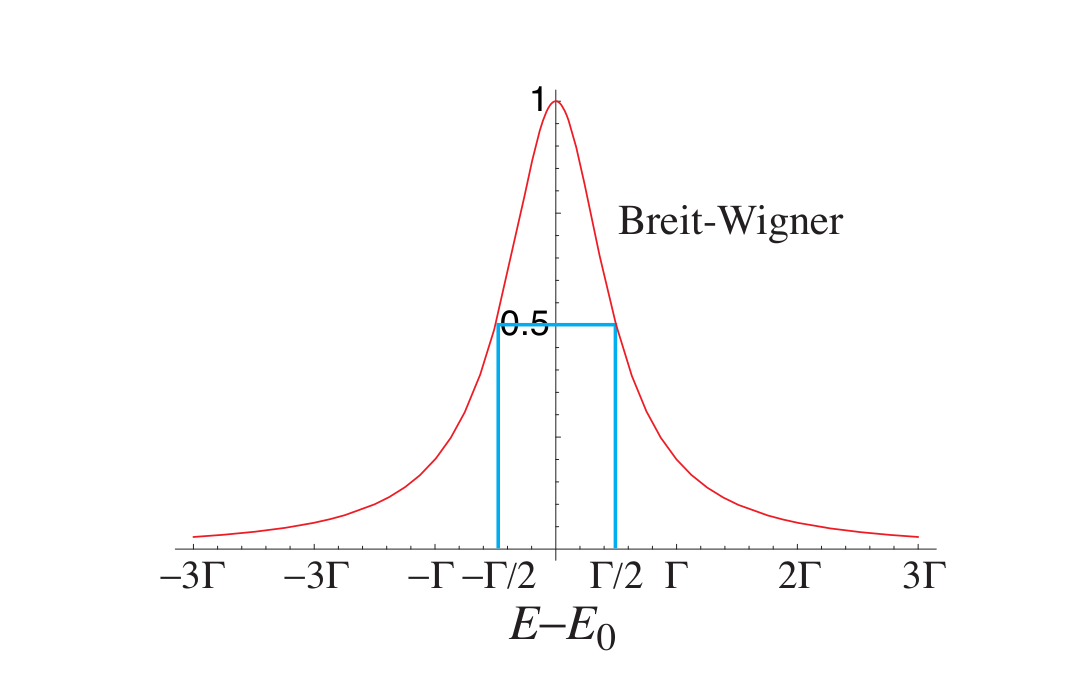
\includegraphics[height=4cm ,width=6.23cm]{QM/resonance.png}
	\caption{Resonance curve}
\end{figure}\\
We then can establish the relationship between the life time of the quasi-bound state and the FWHM of the resonance
\[\tau \Delta E \sim 1\]

\section{Two-to-two scattering}
Similar to the discussion in hydrogen atom, we take as independent variables the center of mass and relative coordinates of the particles
\[\bm{X} = \frac{m_1\bm{x}_1 + m_2\bm{x}_2}{m_1+m_2} \quad \bm{x} = \bm{x}_1-\bm{x}_2\]
The corresponding momentum operators are
\[\bm{P} = \bm{p}_1 + \bm{p}_2 \quad \bm{p} = \frac{m_1\bm{p}_1-m_2\bm{p}_2}{m_1 + m_2}\]
Then the Hamiltonian becomes
\[H = \frac{P^2}{2M} + \frac{p^2}{2\mu} + V(|\bm{x}|)\]
Then the problem reduces to the potential scattering problem for a particle of mass $\mu = \frac{m_1m_2}{m_1+m_2}$.
\\ \\
If two particles that scatter are identical particles, such as electron-electron scattering or scattering of two identical atoms, symmetry of the wave function needs to be considered.
Under the interchange of two particles, the center of mass motion is not affected, but the relative coordinates change their signs. If they have spins, their spins need to be interchanged at the same time.
\\
If two particles are identical spinless bosons, there is no spin degrees of freedom and the interchange of particles is simply $\bm{x} \to -\bm{x}$ in the wave function. 
Because they are bosons, the wave function should not change under the interchange of particles, and hence the wave function must be an even function of $\bm{x}$. 
Therefore the asymptotic form of the wave function must be changed to
\[\psi(\bm{x}) \to e^{ikz} + e^{-ikz} + [f(\theta) + f(\pi - \theta)] \frac{e^{ikr}}{r}\]
The differential cross section is then found to be
\[\frac{d\sigma}{d\Omega} = |f(\theta)+f(\pi-\theta)^2|\]
Note that one should not integrate over the entire solid angle to obtain the total cross section because $(\theta,\phi)$ and $(\pi - \theta,\phi+\pi)$ correspond to an identical state.
\\
For two spin $\frac{1}{2}$ fermions, there are two possible spin wave functions, symmetric $S = 1$ and anti-symmetric $S = 0$.
Therefore depending on the spin wave function, we either have a anti-symmetric or symmetric spatial wave function, respectively. In particular, the differential cross section is the same as the spinless bosons for the anti-symmetric spin wave function $S= 0 $ while it is
\[\frac{d\sigma}{d\Omega} = |f(\theta) - f(\pi-\theta)^2|\]
for the symmetric spin wave function $S = 1$.

\section{Time-dependent formulation}
Recall the time-dependent perturbation theory, the rate of the initial state $|i\rangle$ to transform to the final state $|f\rangle$ to the first order in perturbation $V$ is
\[\Gamma(i \to f) = 2\pi \delta(E_i-E_f) |V_{fi}|^2\]
When applied to the scattering problem, an additional issue is to define how we sum over the final states. 
In particular, we would like to sum over the continuum plane-wave states, and we must make the sum well-defined.
To define the sum over the continuum states, it is useful to consider the system in a cube of size $L$. 
We impose the periodic boundary condition. The plane-wave solutions in this box are given by
\[\psi_{n_x,n_y,n_z}(\bm{x}) = \frac{1}{L^{3/2}} e^{2\pi i(n_x x + n_y y + n_z z)/L}\]
In the limit $L \to \infty$, we have
\[\sum_{n_x,n_y,n_z} = \left( \frac{L}{2\pi}\right)^3 \sum_{n_x,n_y,n_z} \left( \frac{2\pi}{L}\right)^3 \to \left( \frac{L}{2\pi}\right)^3 \int d\bm{p} = \int \frac{d\bm{x}d\bm{p}}{(2\pi)^3}\]
Coming back to the scattering problem, we sum over the final states to define the probability of the outgoing particle to go into various momentum states
\[\sum_{f} \Gamma(i \to f) = \int \frac{L^3 d\bm{p}}{(2\pi)^3} 2\pi \delta(E_i-E_f) |V_{fi}|^2\]
Note that
\[V_{fi} = \int d\bm{x} \frac{e^{-i\bm{p}_f \cdot \bm{x}}}{L^{3/2}} V(\bm{x}) \frac{e^{i\bm{p}_i \cdot \bm{x}}}{L^{3/2}}  = \frac{1}{L^3} \int d\bm{x} V(\bm{x}) e^{i\bm{q}\cdot\bm{x}}\]
where $\bm{q} = \bm{p}_i - \bm{p}_f$.
Since the incident flux of the incoming particle is $\frac{v}{L^3}$, the cross section is
\[\sigma = \frac{L^3}{v} \sum_{f} \Gamma(i \to f) =  \frac{m}{p_i} \int \frac{ d\bm{p}}{(2\pi)^3} 2\pi \delta(E_i-E_f) \left |\int d\bm{x} V(\bm{x}) e^{i\bm{q}\cdot\bm{x}} \right|^2\]
Note that $E = \frac{p^2}{2m}$ and $\delta(E_i-E_f) = \frac{m}{p_i} \delta(p_f-p_i)$, finally we can get
\[\sigma = \int d\Omega \left | \frac{m}{2\pi} \int d\bm{x} V(\bm{x}) e^{i\bm{q}\cdot\bm{x}} \right|^2\]
This is nothing but the Born approximation for the cross section.
